% Full-length research report: every figure and the structured content of README.md,
% arranged as Abstract -> Introduction -> Method -> Results -> Conclusion.
% The 3-page version is proposal.tex. Build: cd docs/proposal && latexmk -pdf report-full.tex
% Numbers come only from README.md; citations from README.md "References", docs/paper/ and
% research_notes/Neurosymbolic world models proposal/.
\documentclass[letterpaper, 10pt, conference]{IEEEtran}
\IEEEoverridecommandlockouts
\usepackage{amsmath,amssymb}
\usepackage{graphicx}
\usepackage{booktabs}
\usepackage{array}
\usepackage{xcolor}
\usepackage{cite}
\usepackage{capt-of}
\usepackage[hidelinks]{hyperref}
\usepackage[scaled=0.92]{helvet}
% Figure format follows the ICRA paper: [!t] placement, plots at 0.5--0.72\columnwidth,
% paired images as [b] minipages in one column, figure* only for wide plots, the large
% screenshot comparison on its own float page, captions of one or two lines.
\setlength{\textfloatsep}{9pt plus 2pt minus 2pt}
\setlength{\dbltextfloatsep}{9pt plus 2pt minus 2pt}
\setlength{\floatsep}{8pt plus 2pt minus 2pt}
\setcounter{topnumber}{4}\setcounter{totalnumber}{6}\setcounter{dbltopnumber}{3}
\graphicspath{{../images/}}
\renewcommand{\topfraction}{0.9}\renewcommand{\dbltopfraction}{0.9}
\renewcommand{\textfraction}{0.07}\renewcommand{\floatpagefraction}{0.8}
\renewcommand{\arraystretch}{1.05}
\newcolumntype{L}[1]{>{\raggedright\arraybackslash}p{#1}}

\newcommand{\applicant}{Ned Pham}   % <- check spelling, then rebuild
\newcommand{\demourl}{https://neural-symbolic-nlp.onrender.com/train-neural-symbolic}
\newcommand{\codeurl}{https://github.com/nhan03bit/neural_symbolic_nlp}

% Header box: abstract (from the literature in docs/paper) and index terms left, Fig. 1 right.
\definecolor{absgray}{gray}{0.92}
\newcommand{\abstracttext}{Neural networks trained by next-word prediction are strong at perception, but keep no explicit link to the rules behind a decision. Sheth, Roy and Gaur argue that safety-critical AI needs knowledge set as guardrails during training, not after it, and sort neurosymbolic methods into \emph{lowering}, which compresses symbolic knowledge into the network, and \emph{lifting}, which maps neural outputs to symbols for reasoning. On the lowering side, the semantic loss of Xu et al.\ turns a logical constraint into a training term. Ahmed et al.\ extend it to autoregressive models, where the exact probability of a constraint is \#P-hard, and on GPT-2 pair it with word banning at decoding. A loss gives no test-time guarantee, and a mask leaves the model unchanged. This report asks what happens when one knowledge base drives both and a verifier lifts the output back to symbols, on a small transformer, and proposes the same split for neurosymbolic world models in robotic manipulation.}
\makeatletter
\let\old@maketitle\@maketitle
\renewcommand{\@maketitle}{\old@maketitle\vspace{-4pt}\setcounter{figure}{0}
\noindent\colorbox{absgray}{\begin{minipage}{\dimexpr\textwidth-2\fboxsep\relax}
\begin{minipage}[c]{0.445\linewidth}\sffamily\small\bfseries
\textit{Abstract}---\abstracttext\par\smallskip
\textit{Index Terms}---Neuro-symbolic AI, lowering and lifting, semantic loss, constrained decoding, knowledge bases, world models, robotic manipulation.
\end{minipage}\hfill
\begin{minipage}[c]{0.535\linewidth}\centering
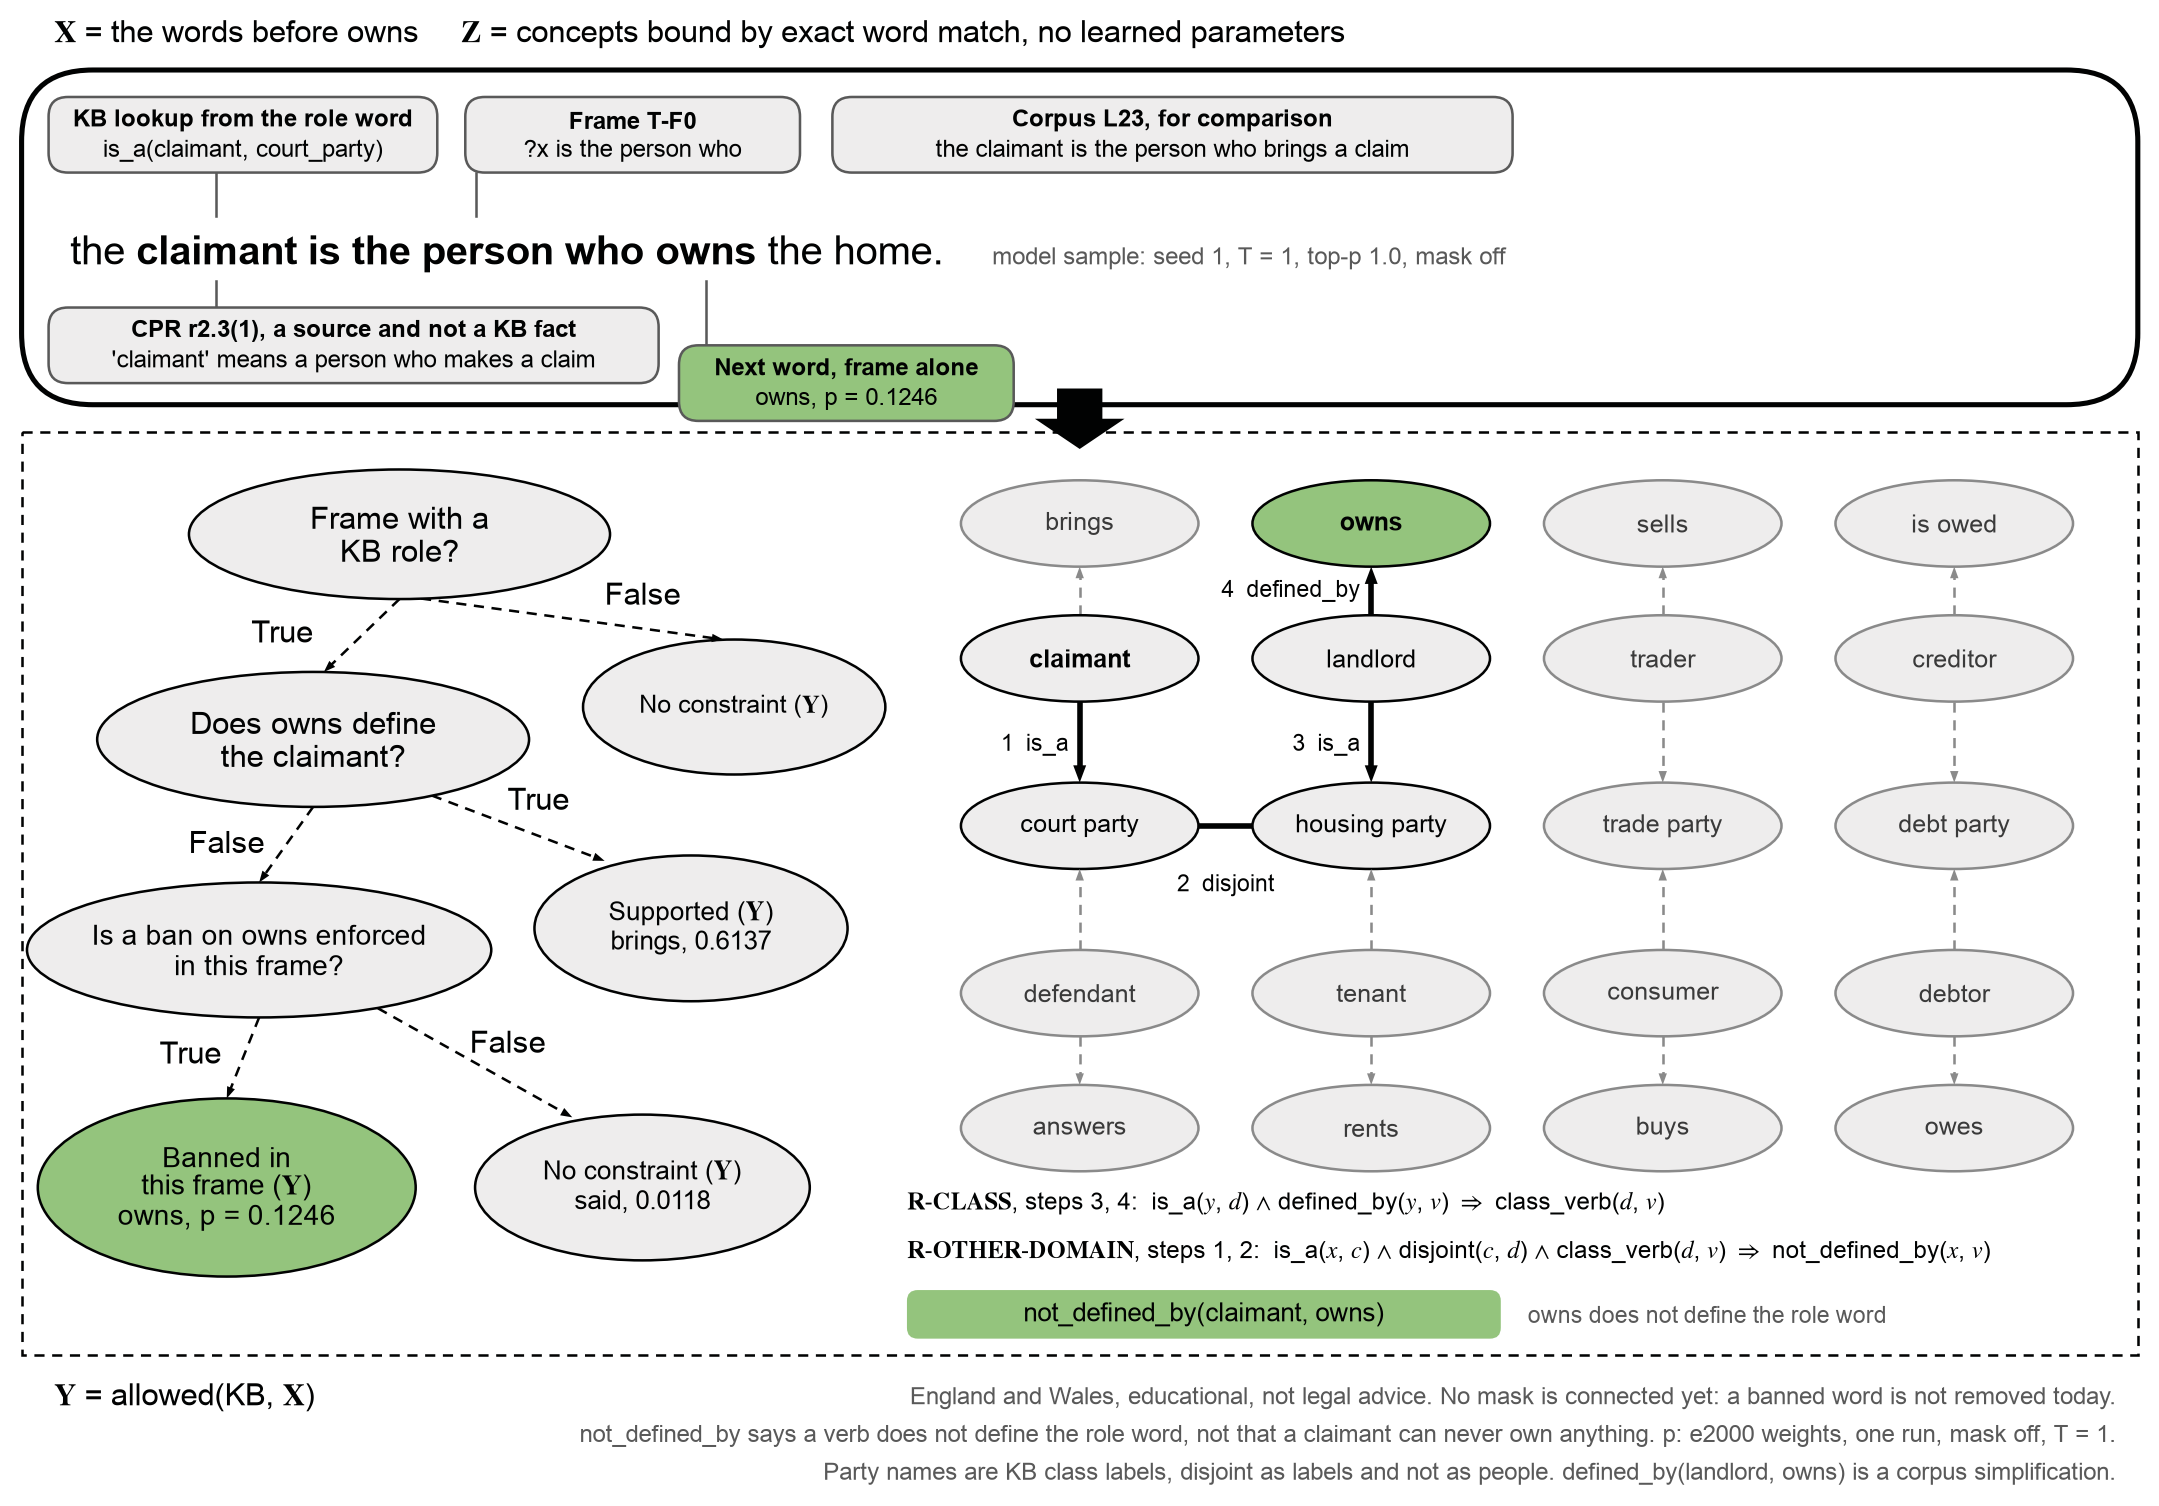
\includegraphics[width=\linewidth,trim=0 48 0 0,clip]{fig-civil-law-kb.png}\\[-2pt]
{\scriptsize\captionof{figure}{\textbf{The core logic.} One sampled sentence, ``the claimant is the person who owns the home'', traced through the civil-law KB: the frame matches, the KB holds a ban on \emph{owns} through \textit{is\_a}, \textit{disjoint}, \textit{is\_a} and \textit{defined\_by}, and \emph{owns} is banned in this frame. Network alone: $p{=}0.1246$ on \emph{owns}, 0.6137 on \emph{brings}. One unmasked sample (seed 1, $T{=}1$, top-$p$ 1.0); educational KB, not legal advice.}\label{fig:logic}}
\end{minipage}
\end{minipage}}\vspace{2pt}}
\makeatother

\title{\LARGE\bf Neural-Symbolic NLP on a Small Transformer:\\Towards Neurosymbolic World Models for Manipulation}

\author{\applicant\thanks{Research report for EPSRC DLA project S3.5-COM-Valentino, University of Sheffield, for Dr Marco Valentino (NLP group) and Dr Amir Ghalamzan. Full-length version; the 3-page version is \texttt{proposal.pdf}. Live demo: \url{\demourl}. Code: \url{\codeurl}.}}

\begin{document}
\maketitle
\thispagestyle{empty}
\pagestyle{empty}

%======================================================================
\section{Introduction}
Foundation models give robots broad priors but no guarantee that a step obeys a rule. Vision-language-action (VLA) policies above 90\% success on standard LIBERO fall to 0.0\% under simple perturbations~\cite{liberopro}. On Towers of Hanoi, a PDDL-based neuro-symbolic system reached 95\% against 34\% for the best fine-tuned VLA~\cite{duggan}.

The same gap appears in language at a scale small enough to inspect. A language model trained on next-token cross-entropy has no notion of truth, because the loss only rewards text that looks like the corpus. Sheth et al.~\cite{sheth2023} frame the remedy as an integration of neural perception with symbolic knowledge, in two families: \emph{lowering} compresses knowledge into the network, and \emph{lifting} extracts neural outputs into symbols for reasoning. For mental-health assistance, they report 70\% expert satisfaction for an intertwined pipeline against 47\% for an LLM in a federated one; the process-knowledge line~\cite{sheth2022,roy2022} argues that such systems must follow, and explain themselves by, the expert's own guideline. On the lowering side, the semantic loss~\cite{xu2018} measures how far the network's output is from satisfying a logical constraint, and the pseudo-semantic loss~\cite{ahmed2023} extends it to autoregressive models.

This project is a from-scratch TypeScript pipeline (no ML libraries) that climbs from a rule-based chatbot to a GPT-style transformer, plus a symbolic layer on top: a knowledge base (KB), a hard logit mask at decoding and a semantic loss in training. \texttt{w3cj/how-llms-work}~\cite{w3cj} is the reference architecture: same five stages, and no code copied. It specifies one pipeline in which the same KB shapes training through a semantic loss and constrains decoding through a hard logit mask. It measures the baselines that motivate the pipeline. One full-length run, at one seed and $\lambda_s{=}50$, has been compared with the baseline; of the planned experiments, E1, E2 and E3 have been run at four training seeds, and E4 without its held-out measures. Every number measured in this project comes from code, not typed in by hand; figures quoted from papers are attributed to them. The status of each stage is in Fig.~\ref{fig:stages} and Table~\ref{tab:stages}.

\begin{figure}[!t]
\centering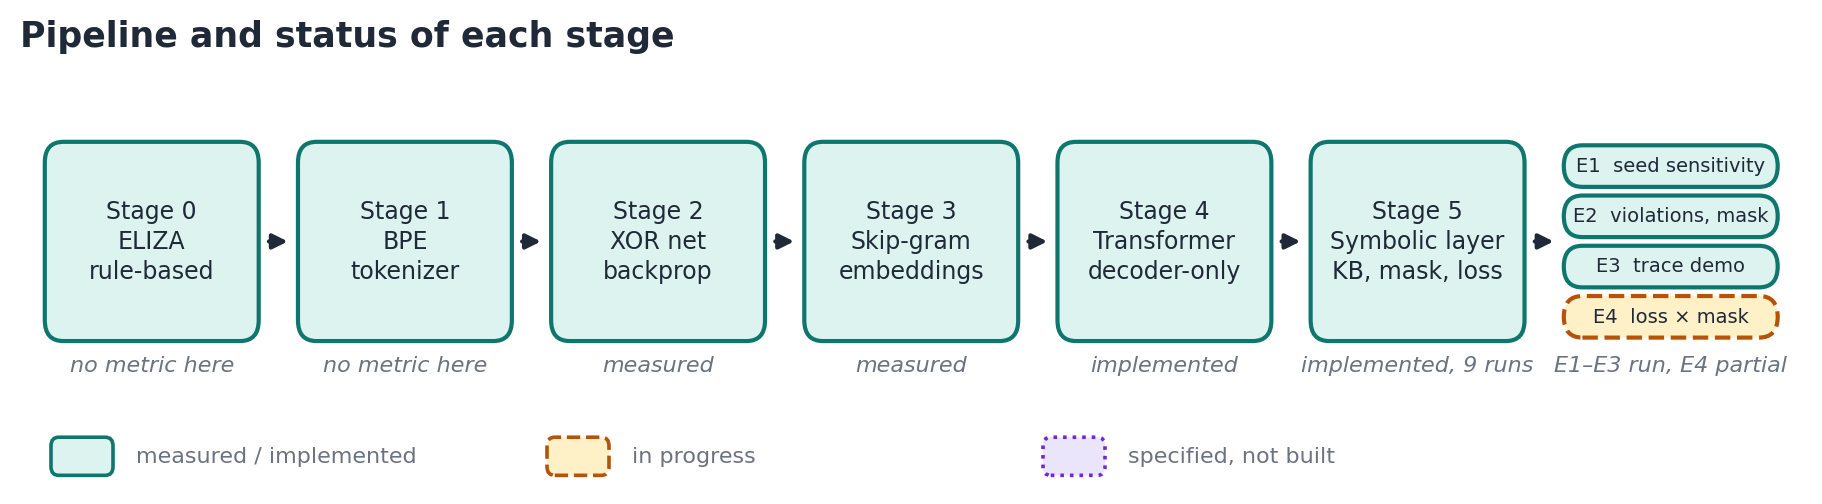
\includegraphics[width=\columnwidth,trim=0 0 0 36,clip]{fig-pipeline.png}
\caption{Pipeline and status of each stage. Teal: built or run; amber: in progress (E4, without held-out measures).}\label{fig:stages}
\end{figure}

\begin{table}[t]
\caption{Stages of the pipeline.}\label{tab:stages}
\centering\footnotesize\setlength{\tabcolsep}{3pt}
\begin{tabular}{@{}cL{2.6cm}L{4.9cm}@{}}
\toprule
Stage & What & State\\
\midrule
0 & ELIZA pattern-matching chat~\cite{weizenbaum} & Works\\
1 & BPE tokenizer~\cite{sennrich} & Works\\
2 & XOR network, 2$\to$4$\to$1 with backprop~\cite{rumelhart} & Works, measured\\
3 & Skip-gram word embeddings~\cite{mikolova,mikolovb} & Fixed (was collapsed), measured\\
4 & Decoder-only transformer~\cite{vaswani} & Done (forward, backward, Adam, top-$p$ generation, multi-threaded training)\\
5 & Symbolic layer & Implemented: KB, hard mask, verifier, semantic loss trainer, lifting. One full-length run, one seed\\
6 & Experiments E1--E4 & E1, E2, E3 run at four training seeds; E4 run except its held-out measures\\
\bottomrule
\end{tabular}
\end{table}

\textbf{Try it.} The demo takes one parameter line, for example \texttt{300 0.8 0.9 2 40 2 42}: epochs, temperature, top-$p$, layers, max tokens, $\lambda_s$ and seed. It trains on the server and streams every epoch. Send \texttt{2000 0.8 0.9 2 40 50 42} to replay the full-length run from its saved weights. The free host sleeps when idle, so the first request can take a minute or more.

%======================================================================
\section{Method}
\subsection{The transformer}
Each token gets a query, key and value; attention weights are $\mathrm{softmax}(QK^\top/\sqrt{d_k}+M)V$ with a causal mask $M$; several heads run in parallel; a feed-forward net refines each token; blocks stack (Fig.~\ref{fig:qkv}). The block is pre-LayerNorm~\cite{ba2016}, as built in GPT-2 (Fig.~\ref{fig:block}):
\begin{align*}
x' &= x + \mathrm{MHA}(\mathrm{LN}_1(x)),\\
x'' &= x' + W_2\,\mathrm{ReLU}(W_1\,\mathrm{LN}_2(x') + b_1) + b_2.
\end{align*}
Config: context 32 (training windows of 16 tokens), $d{=}32$, 2 heads, feed-forward width 128, 1--6 layers (default 2), Adam~\cite{kingma} lr 0.001, one full-batch step per epoch. That is \textbf{12,704 parameters per block}. With the whole-word BPE vocabulary built from the civil-law text (937 tokens, 1781 merges) the model has 87,401 parameters at 2 layers and 138,217 at 6. Training signal is next-token cross-entropy, nothing else. The implementation is in Table~\ref{tab:impl}.

\begin{figure}[!t]
\centering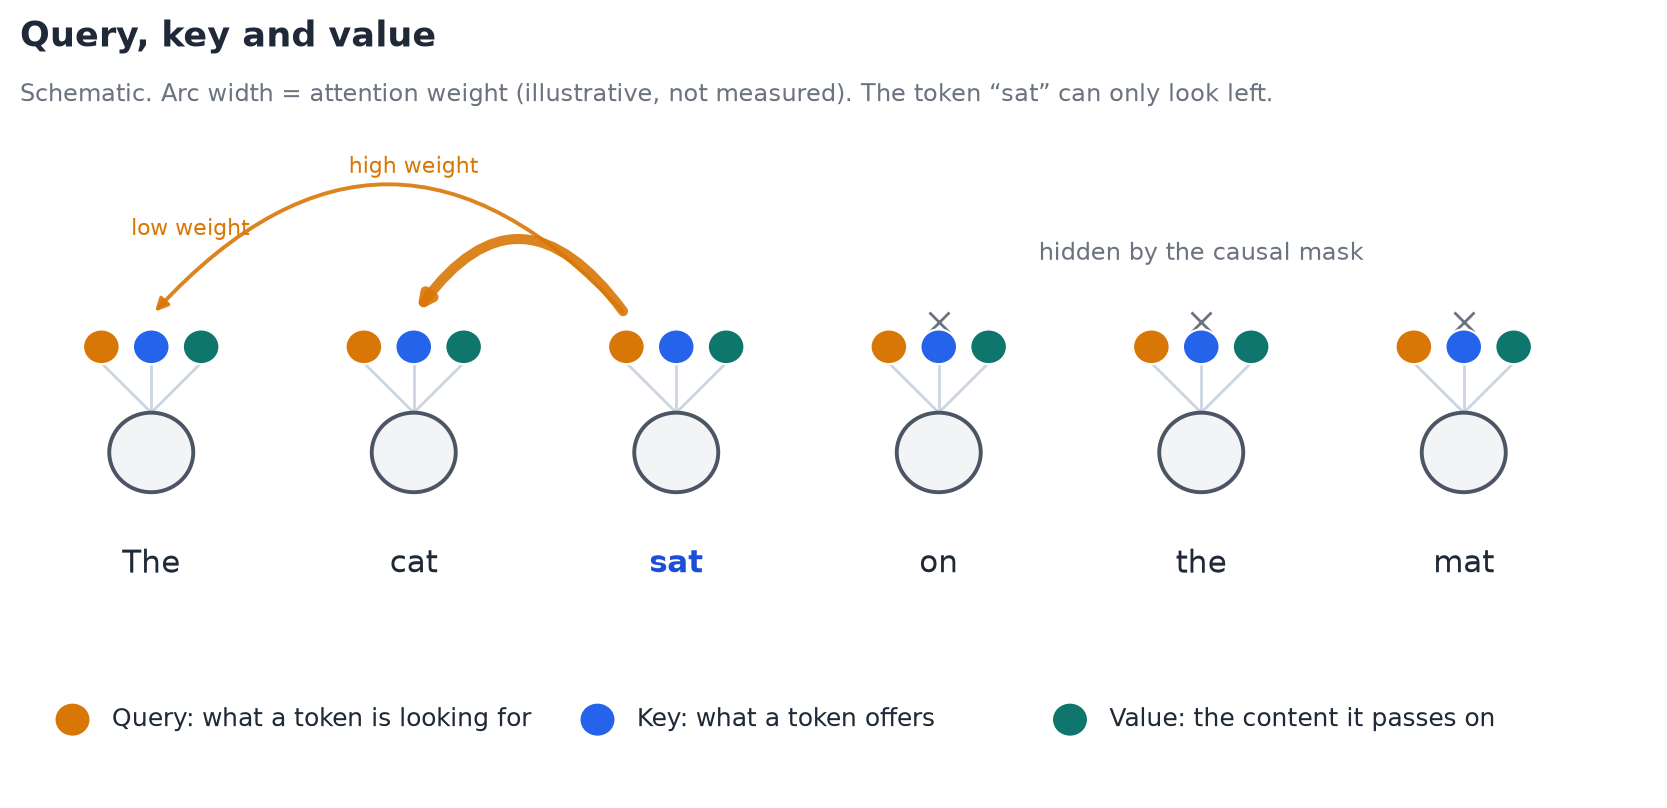
\includegraphics[width=0.92\columnwidth,trim=0 12 0 0,clip]{fig-attn-qkv.png}
\caption{Query, key and value (schematic).}\label{fig:qkv}
\end{figure}

\begin{figure}[!t]
\centering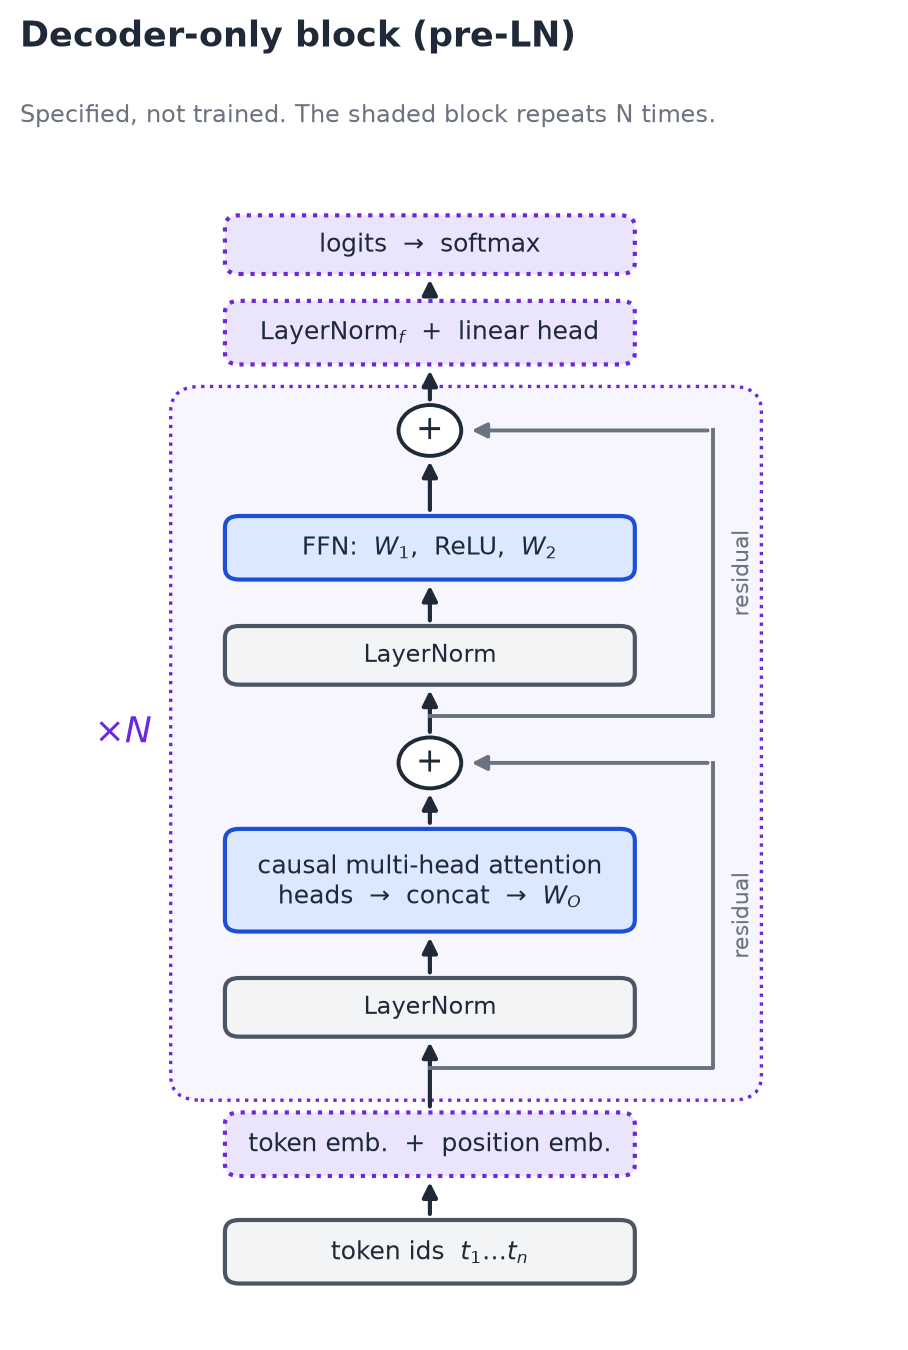
\includegraphics[width=0.5\columnwidth]{fig-transformer-block.png}
\caption{Transformer block (pre-LN, as in GPT-2).}\label{fig:block}
\end{figure}

\begin{table}[t]
\caption{Implementation, in \texttt{src/routes/train-transformer/}.}\label{tab:impl}
\centering\footnotesize\setlength{\tabcolsep}{3pt}
\begin{tabular}{@{}>{\scriptsize}L{2.4cm}L{5.9cm}@{}}
\toprule
File & Role\\
\midrule
\texttt{matrix.ts} & \texttt{matmul}, \texttt{matmulTransA/B}, Xavier init, seeded \texttt{rand} on flat row-major \texttt{Float32Array}s\\
\texttt{transformer.ts} & LayerNorm, causal multi-head attention, FFN, block forward/backward, cross-entropy, Adam, top-$p$ generation\\
\texttt{weigth-layout.ts} & Packs all weights into one \texttt{Shared\-Array\-Buffer}; zero-copy views for every thread\\
\texttt{train-worker.ts} & Worker thread: forward + backward on its slice of sequences, gradients into shared memory\\
\texttt{train.ts} & BPE vocab, sliding windows, spawns \texttt{cpus}$-$2 workers, sums gradients, Adam step, samples, checkpoints every 100 epochs\\
\texttt{index.ts} & \texttt{POST /train-transformer}, streams \texttt{init}, \texttt{epoch} and \texttt{done} events over SSE\\
\bottomrule
\end{tabular}
\end{table}

\textbf{Verification gates} (5 pass): finite-difference gradient check (error $<10^{-3}$), initial loss $\approx\ln V$, overfit a single sequence, causal-mask test, same seed gives same weights. \textbf{Bugs found and fixed.} The gates needed three forward/backward fixes in \texttt{transformer.ts}, made on 2026-11-02: the first residual multiplied instead of adding, attention skipped the token itself ($j<i$), and the gradient for $K$ used $K$ instead of $Q$. Older weights stay on disk but are not loaded, because filenames now carry the model version.

\subsection{One knowledge base, two integration points}
The two designs are not alternatives. A KB of triples plus Horn rules gives one allowed set $A_t$ per position, and that set is used twice (Fig.~\ref{fig:pipe}). Training shapes the distribution, so the model should learn to put little mass on banned tokens. Decoding guarantees the covered cases at test time. The published name for this pattern is constrained learning plus constrained inference. The closest published precedent is Ahmed, Chang and Van den Broeck~\cite{ahmed2023}, on GPT-2 (124M parameters) and RealToxicityPrompts: a pseudo-semantic loss with domain-adaptive training, then Word Banning at decoding. The combination has the lowest toxicity: 9.20\% over all prompts, against 9.80\% without banning and 14.05\% for domain-adaptive training alone. Two differences matter: they score toxicity with the Perspective API rather than the constraint itself, and their loss works around a model sample, whereas the semantic loss here is a per-position term on corpus prefixes.

\begin{figure}[!t]
\centering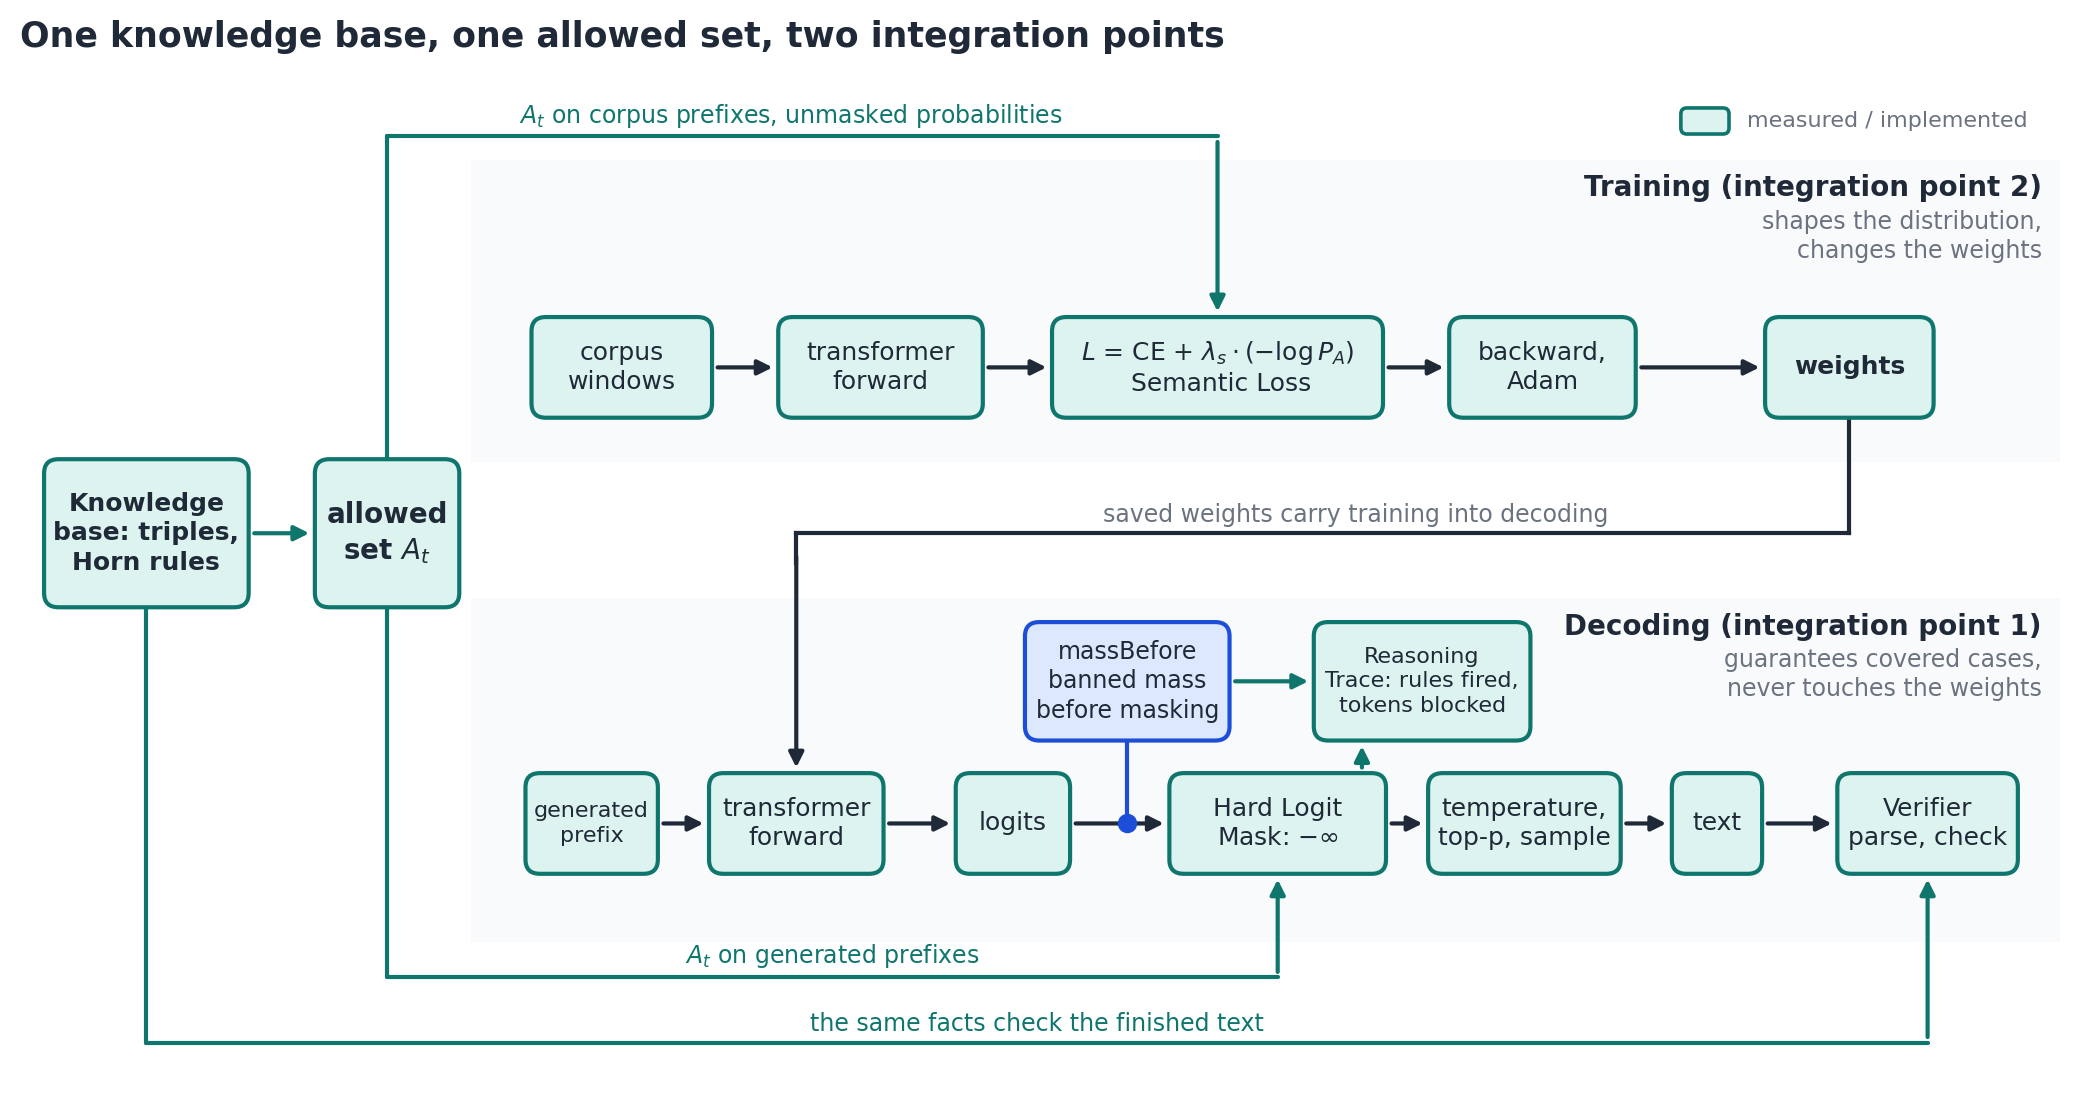
\includegraphics[width=\columnwidth]{fig-design-pipeline.png}
\caption{One KB gives one allowed set, used by the semantic loss in training and by the hard mask at decoding; \textit{massBefore} marks where the trained model meets the mask.}\label{fig:pipe}
\end{figure}

The KB covers definitions in the civil-law corpus, for example
\[\begin{aligned}&\mathit{counterpart}(\mathrm{claimant},\mathrm{defendant})\\&\quad\wedge\mathit{defined\_by}(\mathrm{defendant},\mathrm{answers})\\&\qquad\Rightarrow\mathit{not\_defined\_by}(\mathrm{claimant},\mathrm{answers}).\end{aligned}\]
Forward chaining closes the KB once, and a trigger turns a derived fact into banned token IDs when the context ends in a frame such as ``the claimant is the person who''. Every ban can be printed as a proof. Fig.~\ref{fig:logic} traces one unmasked sample from the saved model (seed 1, $T{=}1$, top-$p$ 1.0), which began ``the claimant is the person who owns the home'', where the corpus says ``brings a claim''. The frame \textit{?x is the person who} binds \emph{claimant}, and the closed KB holds \textit{not\_defined\_by}(claimant, owns) by R-OTHER-DOMAIN, so \emph{owns} is banned. Class labels such as \textit{court\_party} are the KB's own, pairwise disjoint as labels and not as people; \textit{defined\_by}(landlord, owns) is a corpus simplification. These are read-only probes, not a measured effect: with the frame alone and the mask off, \emph{owns} has $p{=}0.1246$, and 265 of 2,000 sampling seeds drew it at top-$p$ 1.0; at top-$p$ 0.6 all 2,000 drew \emph{brings}. A test on the real corpus and tokenizer shows the triggers fire at 9 of 5,390 positions and never ban the next token in the corpus. The layout follows Sheth et al.~\cite{sheth2023}, Fig.~4, and the drawing is original.

\textbf{Method 1: the KB enforced at decoding (hard logit mask).} At each step, the logits of banned token IDs are set to $-\infty$ before temperature and top-$p$. Optional companions are the M2 soft bias (towards supported tokens), the M3 reasoning trace (rules fired, tokens blocked and \textit{massBefore}) and the M4 verifier (parses finished text into triples and checks them).
\begin{itemize}
\item \emph{Guarantee.} Zero mass on covered banned tokens, but only relative to KB coverage, only for whole-word token IDs, and only when a trigger fires.
\item \emph{Limits.} It does not change the weights or choose among allowed tokens. A wrong rule is enforced absolutely. Errors concentrate in the translation from text to logic, so the verifier reports only on what it could parse.
\item \emph{Taxonomy.} In~\cite{sheth2023} this is 1a-style lowering, by analogy, not strict 1a: the knowledge is neither compressed nor learned. The mapping is ours.
\end{itemize}

\textbf{Method 2: semantic loss in training.} The objective is $L=\mathrm{CE}+\lambda_s(-\log P_A)$, where $P_A$ is the probability mass on allowed tokens (\cite{xu2018}; the categorical form is~\cite{ahmed2023}, Eq.~3). It is a deterministic function of the logits; the randomness comes from seeded initialisation and top-$p$ sampling, and this term leaves both in place.
\begin{itemize}
\item \emph{It cannot see the choice among allowed tokens.} $H(p)=H_b(P_A)+P_AH(q_A)+(1{-}P_A)H(q_B)$, where $q_A$ and $q_B$ are $p$ renormalised over allowed and banned tokens. The loss depends only on $P_A$, so $H(q_A)$ is outside its objective (our derivation). A constraint ``only specifies what worlds are possible but does not specify which one is correct''~\cite{vankrieken}.
\item \emph{It is a soft penalty.} Where data and rule conflict, the optimum at one context keeps banned mass $f_B/(1+\lambda_s)$, where $f_B$ is the banned tokens' frequency in the data (our derivation). There is no test-time guarantee~\cite{ahmed2022}.
\item \emph{It acts only where it is applied.} Where the target is allowed, $\mathrm{CE}=\text{masked CE}+(-\log P_A)$, so the term changes the speed of learning there, not the optimum (our derivation). It fires at 86 of 85,984 training-window positions (0.100\%), with the target allowed at all of them, so a null result is plausible.
\item \emph{It may amplify seed differences.} Zombori et al.~\cite{zombori}, Theorem~4, prove for softmax regression that, with no other supervision, this form of loss concentrates mass on whichever allowed token starts largest. Whether that happens in a transformer has to be measured.
\item \emph{Taxonomy.} Towards 2b (intertwined), not end-to-end differentiable reasoning: the KB is discrete and only the loss term is differentiable. Sheth et al.\ do not use the term ``semantic loss'', so this placement is also our reading.
\end{itemize}

\textbf{Why the semantic loss needs the mask.}
\begin{itemize}
\item \emph{Violation rate cannot show what the loss adds.} With the mask on, violations of token-expressible rules should be 0 by construction; E4 found one surface form the mask does not cover (``owed'', Sec.~\ref{sec:e14}). So the evaluation reads its contribution from \textit{massBefore}, violations with the mask off, violations the verifier finds that a token mask cannot express, and held-out cross-entropy on targets that do not conflict with the KB.
\item \emph{Prediction, not a result.} A model trained with the loss puts less mass on banned tokens (P5), so the mask has to intervene less. The distortion at one context is $KL(q_A\Vert p)=-\log P_A$, the value of the semantic loss there (our derivation). A covered context still samples from $q_A$, so no finite $\lambda_s$ makes the mask unnecessary for a correct rule.
\item \emph{Shared failure mode.} A wrong or missing rule enters both stages at once. If lifting were ever allowed to add bans, a wrong accepted triple would reach both stages, so that step stays off.
\item \emph{Perplexity cost.} A hard mask gives infinite perplexity on reference text containing a banned token~\cite{ahmed2023}. Here, E2 computes perplexity from the weights alone, and E4 reports held-out cross-entropy on targets that do not conflict with the KB.
\end{itemize}
The stated target stays \textbf{zero mass on rule-excluded tokens and a calibrated spread over the rest}, with each guarantee stated next to its coverage.

\subsection{Mechanisms and the taxonomy}
In the terms of Sheth et al.~\cite{sheth2023}, \textbf{lowering} compresses symbolic knowledge into the neural side, \textbf{lifting} lifts neural output into symbols (Fig.~\ref{fig:tax}, Table~\ref{tab:mech}, Fig.~\ref{fig:flow}). A mask is not understanding: it blocks a class of outputs and leaves the weights unchanged. The trace explains the symbolic decision, not the network's internal computation.

\begin{figure*}[!t]
\centering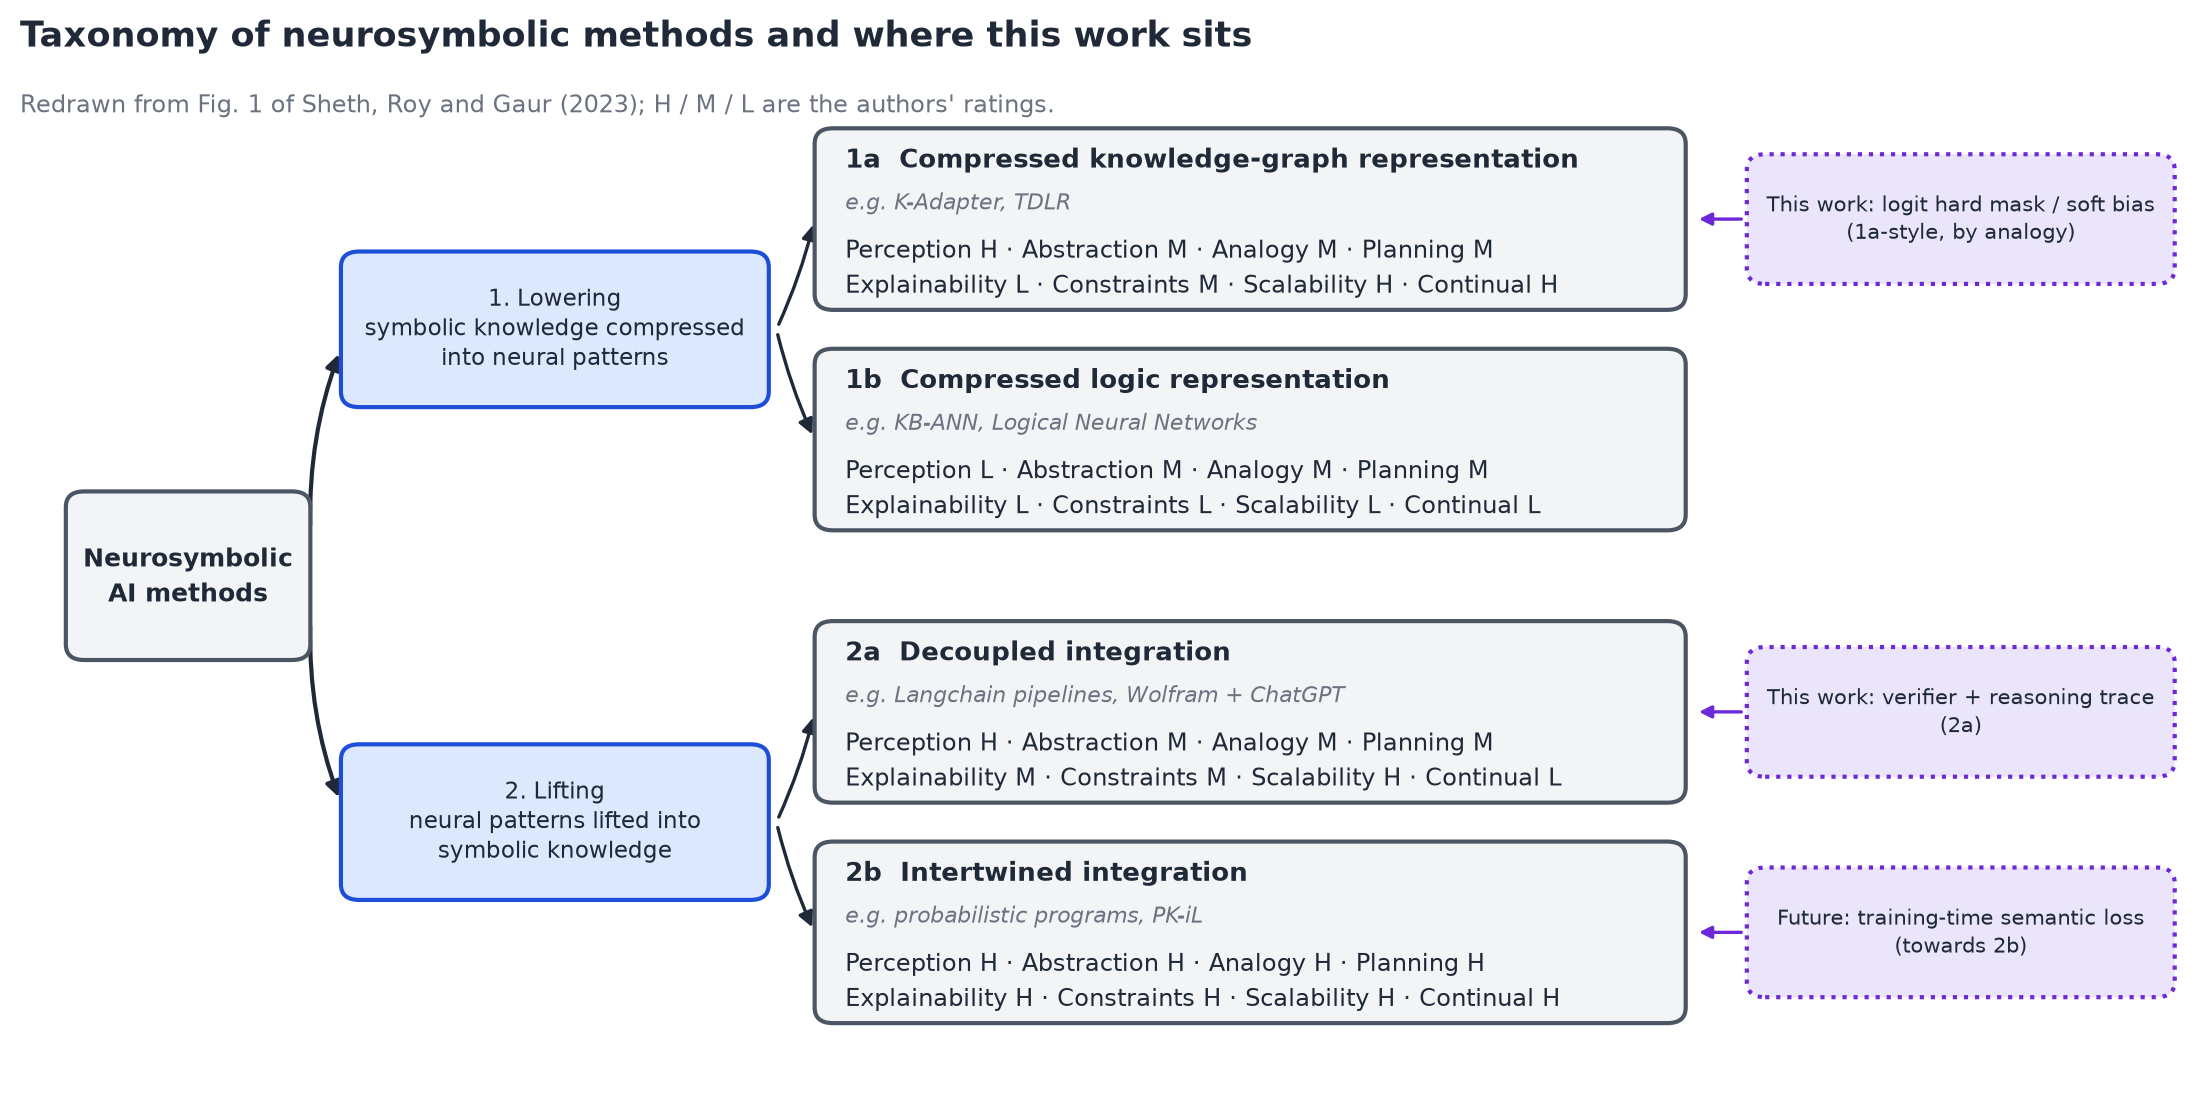
\includegraphics[width=0.66\textwidth]{fig-taxonomy-mapping.png}
\caption{Taxonomy mapping, redrawn from~\cite{sheth2023}, Fig.~1 (H/M/L: its authors' ratings). \emph{Status note:} the ``Future'' semantic loss is now implemented.}\label{fig:tax}
\end{figure*}

\begin{table}[t]
\caption{Mechanisms and their position in the taxonomy.}\label{tab:mech}
\centering\footnotesize\setlength{\tabcolsep}{3pt}
\begin{tabular}{@{}L{1.7cm}L{4.1cm}L{2.3cm}@{}}
\toprule
Mechanism & What it does & Position\\
\midrule
M1 Hard logit mask & Sets logits of KB-violating tokens to $-\infty$ before temperature and softmax & 1a-style lowering, by analogy\\
M2 Soft bias & Adds $+\lambda$ to tokens the KB supports & 1a-style lowering, by analogy\\
M3 Reasoning trace & Per step: rules fired, tokens blocked, mass before and after & Part of 2a\\
M4 Verifier & Parses generated text into triples, checks them against the KB & 2a decoupled lifting\\
M5 Semantic loss & Training term rewarding mass on allowed tokens & Toward 2b\\
\bottomrule
\end{tabular}
\end{table}

\begin{figure}[!t]
\centering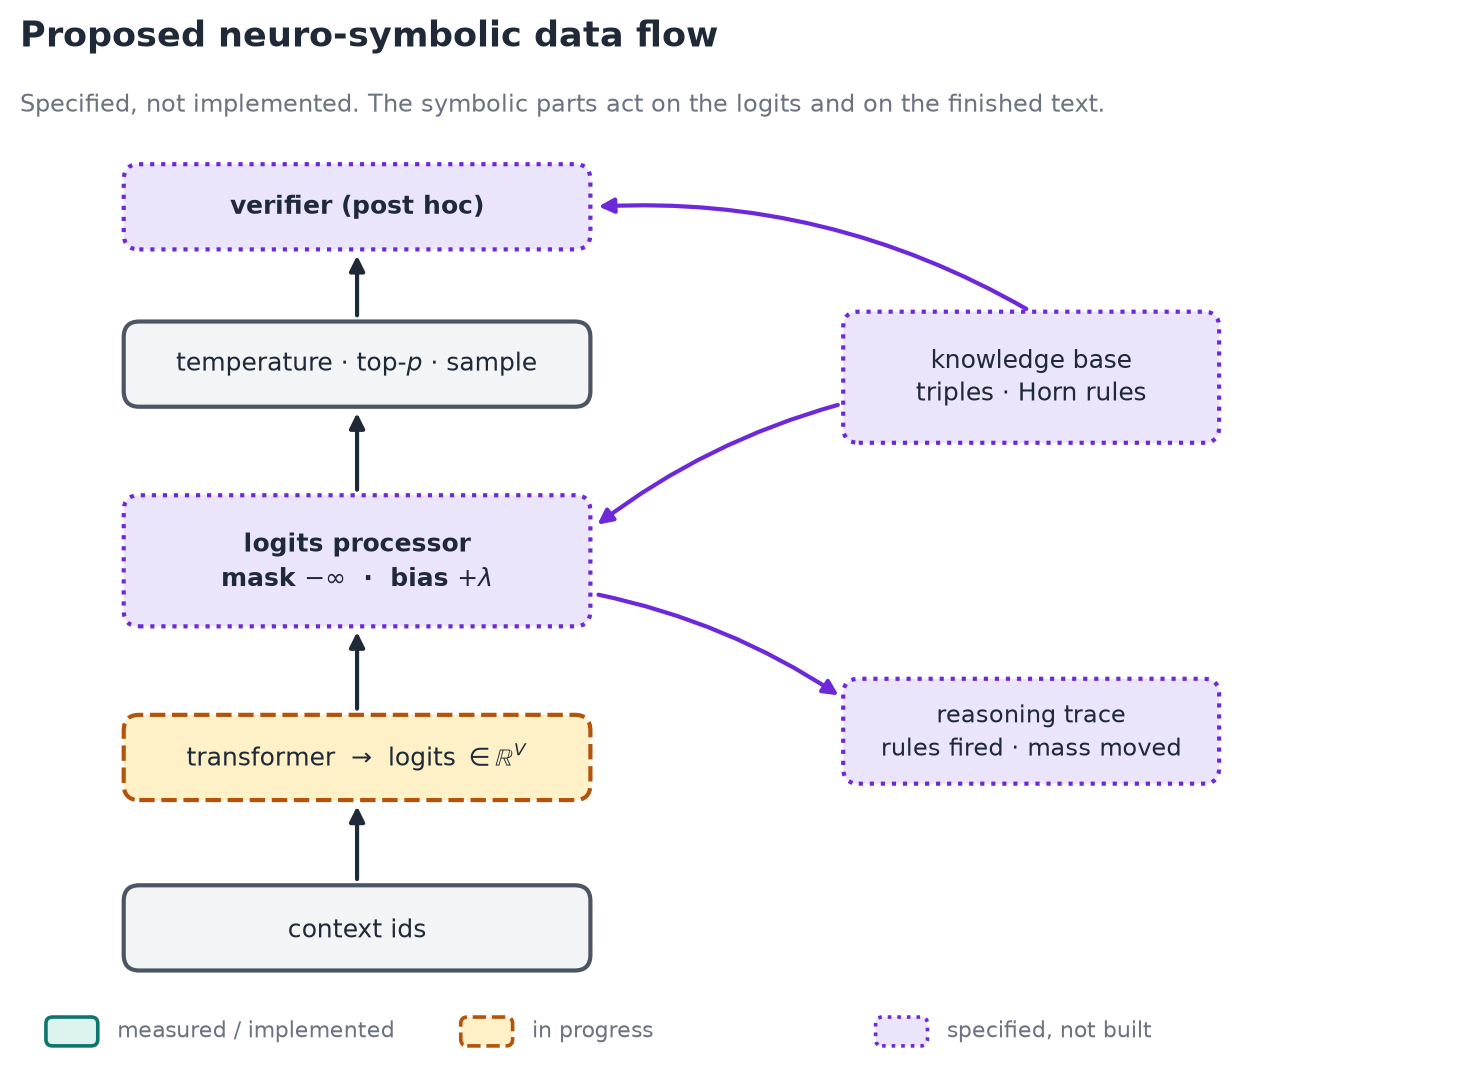
\includegraphics[width=0.72\columnwidth]{fig-neurosymbolic-flow.png}
\caption{Data flow at decoding. \emph{Status note:} the parts marked ``specified, not built'' are now implemented.}\label{fig:flow}
\end{figure}

\subsection{Lifting: network patterns into symbolic knowledge}
This is the ``neural patterns lifted into symbolic knowledge'' half of the design. It probes the trained network with templates, reads its next-word distribution and turns confident verb predictions into \textbf{candidate} triples (Table~\ref{tab:lift}). \textbf{Reported only.} The neural-symbolic trainer runs lifting at every epoch and shows each candidate's status, but a \emph{novel} word that passes the gate is only flagged, never added to the KB. An accepted triple is the network's belief, not ground truth, and it would stay out of the mask and the semantic loss.

\begin{table}[t]
\caption{Lifting: status of a candidate triple.}\label{tab:lift}
\centering\footnotesize\setlength{\tabcolsep}{3pt}
\begin{tabular}{@{}L{1.2cm}L{2.6cm}L{4.4cm}@{}}
\toprule
Status & Meaning & Action\\
\midrule
confirmed & KB already holds it & None. Evidence the network learned the fact, though on this model it may be memorisation\\
conflict & KB derives the opposite (\textit{not\_defined\_by}) & Report with probability and proof. Direct evidence of the reasoning gap\\
novel & Neither & Accept only if $p\ge\tau$ \textbf{and} it creates no new contradiction\\
\bottomrule
\end{tabular}
\end{table}

\subsection{Two separate trainers}
The baseline and the neural-symbolic model are trained apart, so the difference between them can be inspected directly (Table~\ref{tab:trainers}). They share the corpus, tokeniser, model code, Adam and hyperparameters; only the loss differs. The compare view runs both models on one prompt and sampling seed, with the mask off and on, and shows their text, the mask trace, the verifier's claim counts and the banned mass at each definition frame. A test shows that at $\lambda_s{=}0$ and seed 42 the new trainer saves the baseline's weights and losses, so $\lambda_s{=}0$ is the CE-only control at seeds the baseline does not offer.

\begin{table}[t]
\caption{The two trainers.}\label{tab:trainers}
\centering\footnotesize\setlength{\tabcolsep}{3pt}
\begin{tabular}{@{}l>{\scriptsize}L{3.0cm}>{\scriptsize}L{3.9cm}@{}}
\toprule
 & Baseline & Neural-symbolic\\
\midrule
Code & \texttt{train-transformer/\allowbreak train.ts} & \texttt{neural-symbolic/\allowbreak train.ts}\\
Page & \texttt{/train-transformer} & \texttt{/train-neural-symbolic}\\
Loss & CE & CE $+\lambda_s(-\log P_A)$\\
Seed & 42 only & Chosen per run\\
Weights & \texttt{transformer-weights-*} & \texttt{neural-symbolic-\allowbreak weights-*}, named with $\lambda_s$, seed and KB hash\\
\bottomrule
\end{tabular}
\end{table}

\subsection{Falsifiable predictions and planned experiments}
P1 and P2 follow from the construction, so they test the implementation; P3--P7 are empirical and may fail (Table~\ref{tab:pred}). Table~\ref{tab:exp} lists what each experiment has and still needs.

\begin{table}[t]
\caption{Falsifiable predictions.}\label{tab:pred}
\centering\footnotesize\setlength{\tabcolsep}{3pt}
\begin{tabular}{@{}lL{3.9cm}lL{2.6cm}@{}}
\toprule
\# & Prediction & Test & Refuted if\\
\midrule
P1 & With the hard mask on, the violation rate is 0 for token-expressible constraints & E2 & any such violation\\
P2 & With the processor off, output equals the unconstrained baseline at the same seed & unit test & any difference\\
P3 & The unconstrained model violates the KB at a non-trivial rate & E2 & rate near 0\\
P4 & Seeds give similar loss but different weights & E1 & seeds agree closely in weights\\
P5 & Semantic loss lowers the network's own forbidden mass & E4 & not lower, mask off\\
P6 & Semantic loss reduces solution ambiguity across seeds but not weight ambiguity & E4 & JS of $(P_A,1{-}P_A)$ does not shrink, or weight cosine near 1\\
P7 & The cost on unconstrained text is small & E4 & large rise in perplexity where no rule fires\\
\bottomrule
\end{tabular}
\end{table}

\begin{table*}[t]
\caption{Experiments: what is in place and what is left.}\label{tab:exp}
\centering\footnotesize\setlength{\tabcolsep}{4pt}
\begin{tabular}{@{}L{3.2cm}L{1.3cm}L{6.4cm}L{5.9cm}@{}}
\toprule
Experiment & Tests & In place now & Left to do\\
\midrule
E1: seed sensitivity & P4 & Run: $\lambda_s{=}0$ at seeds 42, 1, 2 and 3, 2000 epochs & Nothing for P4. Held-out text, not just held-out prompts, needs the held-out split\\
E2: violation rate, mask off/on & P1, P3 & Run at training seeds 42, 1, 2, 3 (the $\lambda_s{=}0$ models), 24 prompts $\times$ 50 sampling seeds, mask off and on & Perplexity from the weights alone on held-out text. Close the ``owed'' gap in the mask or the verifier, then re-run\\
E3: one full trace & --- & Run: one generation's trace for both models & Nothing\\
E4: loss $\times$ mask ablation & P5, P6, P7 & Run: $\lambda_s\in\{0,2\}$ $\times$ mask off/on $\times$ seeds 42, 1, 2, 3, 2000 epochs, probe contexts outside training and a frequency-matched control set & A held-out split in the neural-symbolic trainer, a held-out KB, and held-out cross-entropy (P7 here is measured on training text)\\
\bottomrule
\end{tabular}
\end{table*}

%======================================================================
\section{Results}\label{sec:results}
\subsection{Baselines before the symbolic layer}
Everything in this subsection was trained by next-token or context prediction alone, with \textbf{no} KB, mask, bias, trace, verifier or semantic loss.

\textbf{XOR: same function, unrelated weights.} A single layer cannot learn XOR (loss 0.2845 $\to$ 0.2842). A 2$\to$4$\to$1 network can (Table~\ref{tab:xor}, Fig.~\ref{fig:xor}). At 5000 epochs all seeds compute the same function, but the first hidden unit's weights differ completely, for example $[5.84,-1.49,6.18,-0.28]$ for seed 42 against $[0,-6.50,-1.93,5.29]$ for seed 1.

\begin{table}[t]
\caption{XOR, four seeds, same data and settings (final MSE).}\label{tab:xor}
\centering\footnotesize\setlength{\tabcolsep}{4pt}
\begin{tabular}{@{}lrrrr@{}}
\toprule
Epochs & Seed 42 & Seed 1 & Seed 2 & Seed 3\\
\midrule
500 & 0.0144 & 0.0227 & \textbf{0.1506} (not conv.) & 0.0110\\
5000 & 0.00028 & 0.00027 & 0.00031 & 0.00022\\
\bottomrule
\end{tabular}
\end{table}

\begin{figure}[!t]
\centering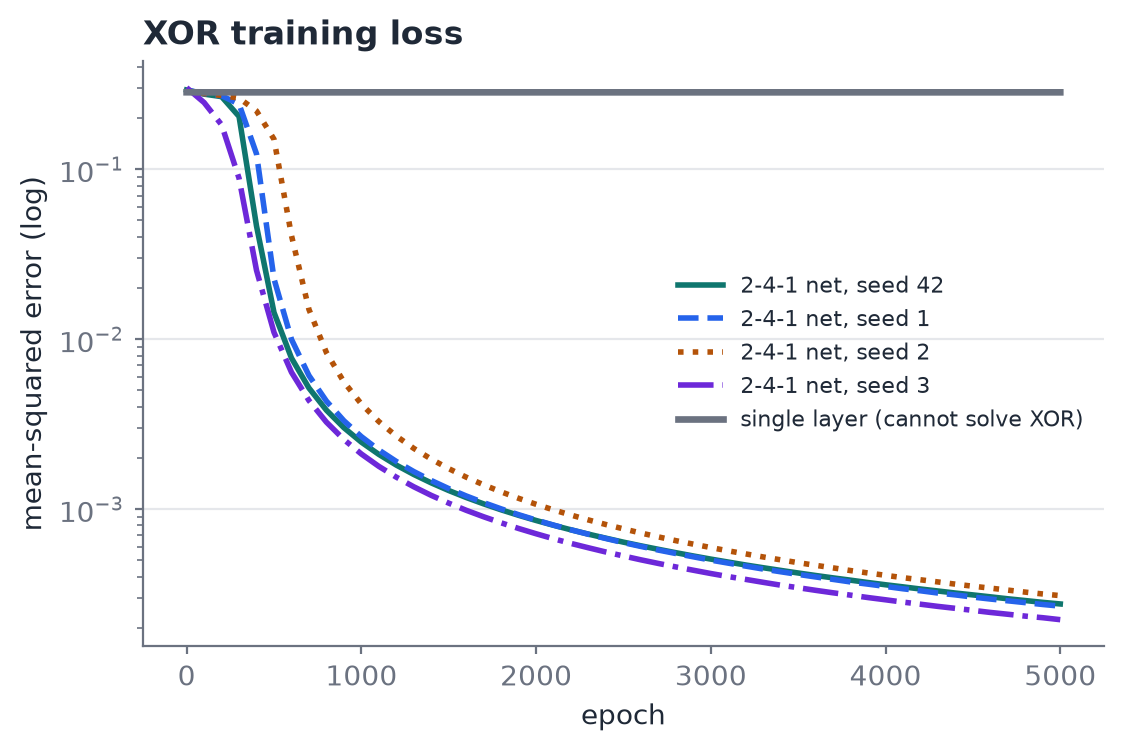
\includegraphics[width=0.72\columnwidth]{fig-xor-loss.png}
\caption{XOR loss and weights across seeds.}\label{fig:xor}
\end{figure}

\textbf{Skip-gram: the civil-law vocabulary, and a wrong answer.} The first version gave every word pair cosine 1.0. Five independent bugs were the cause: an off-by-one in the sampling table, a missing positive update, the wrong row updated for negatives, a wrong analogy sign, and a corpus join that never lower-cased. The model now trains only on England \& Wales civil-dispute text (222 definitions plus 34 dispute stories, 401 sentences; vocab 924 whole-word tokens from 5000 BPE merges; dim 32, window 2, 17,142 training pairs; 10,000 epochs; seed 42). Words that share sentences end up close (Table~\ref{tab:sg}, Fig.~\ref{fig:sg}): the consumer-rights roles form one cluster, and the claimant sits next to the creditor because most claims in the corpus are debt claims. But none of the five analogies returns a role word (Table~\ref{tab:analogy}). The model learned co-occurrence, not the relation ``the party who supplies or lends, against the party who receives or owes''.

\begin{table}[t]
\caption{Skip-gram cosines, civil-law corpus.}\label{tab:sg}
\centering\footnotesize\setlength{\tabcolsep}{4pt}
\begin{tabular}{@{}lrlr@{}}
\toprule
Pair & Cosine & Pair & Cosine\\
\midrule
buyer / customer & 0.76 & defendant / tenant & 0.54\\
seller / buyer & 0.74 & claimant / defendant & 0.44\\
claimant / creditor & 0.69 & trader / consumer & 0.42\\
landlord / tenant & 0.59 & trader / court & $-0.02$\\
creditor / debtor & 0.58 & judge / contract & $-0.13$\\
\bottomrule
\end{tabular}
\end{table}

\begin{table}[t]
\caption{Skip-gram analogies: none returns a role word.}\label{tab:analogy}
\centering\footnotesize\setlength{\tabcolsep}{4pt}
\begin{tabular}{@{}llr@{}}
\toprule
Query & Expected & Returned (cosine)\\
\midrule
landlord $-$ tenant $+$ consumer & trader & \emph{renters} (0.57)\\
trader $-$ consumer $+$ tenant & landlord & \emph{return} (0.65)\\
claimant $-$ defendant $+$ debtor & creditor & \emph{whether} (0.61)\\
creditor $-$ debtor $+$ defendant & claimant & \emph{between} (0.58)\\
seller $-$ buyer $+$ customer & supplier & \emph{proves} (0.72)\\
\bottomrule
\end{tabular}
\end{table}

\begin{figure}[!t]
\centering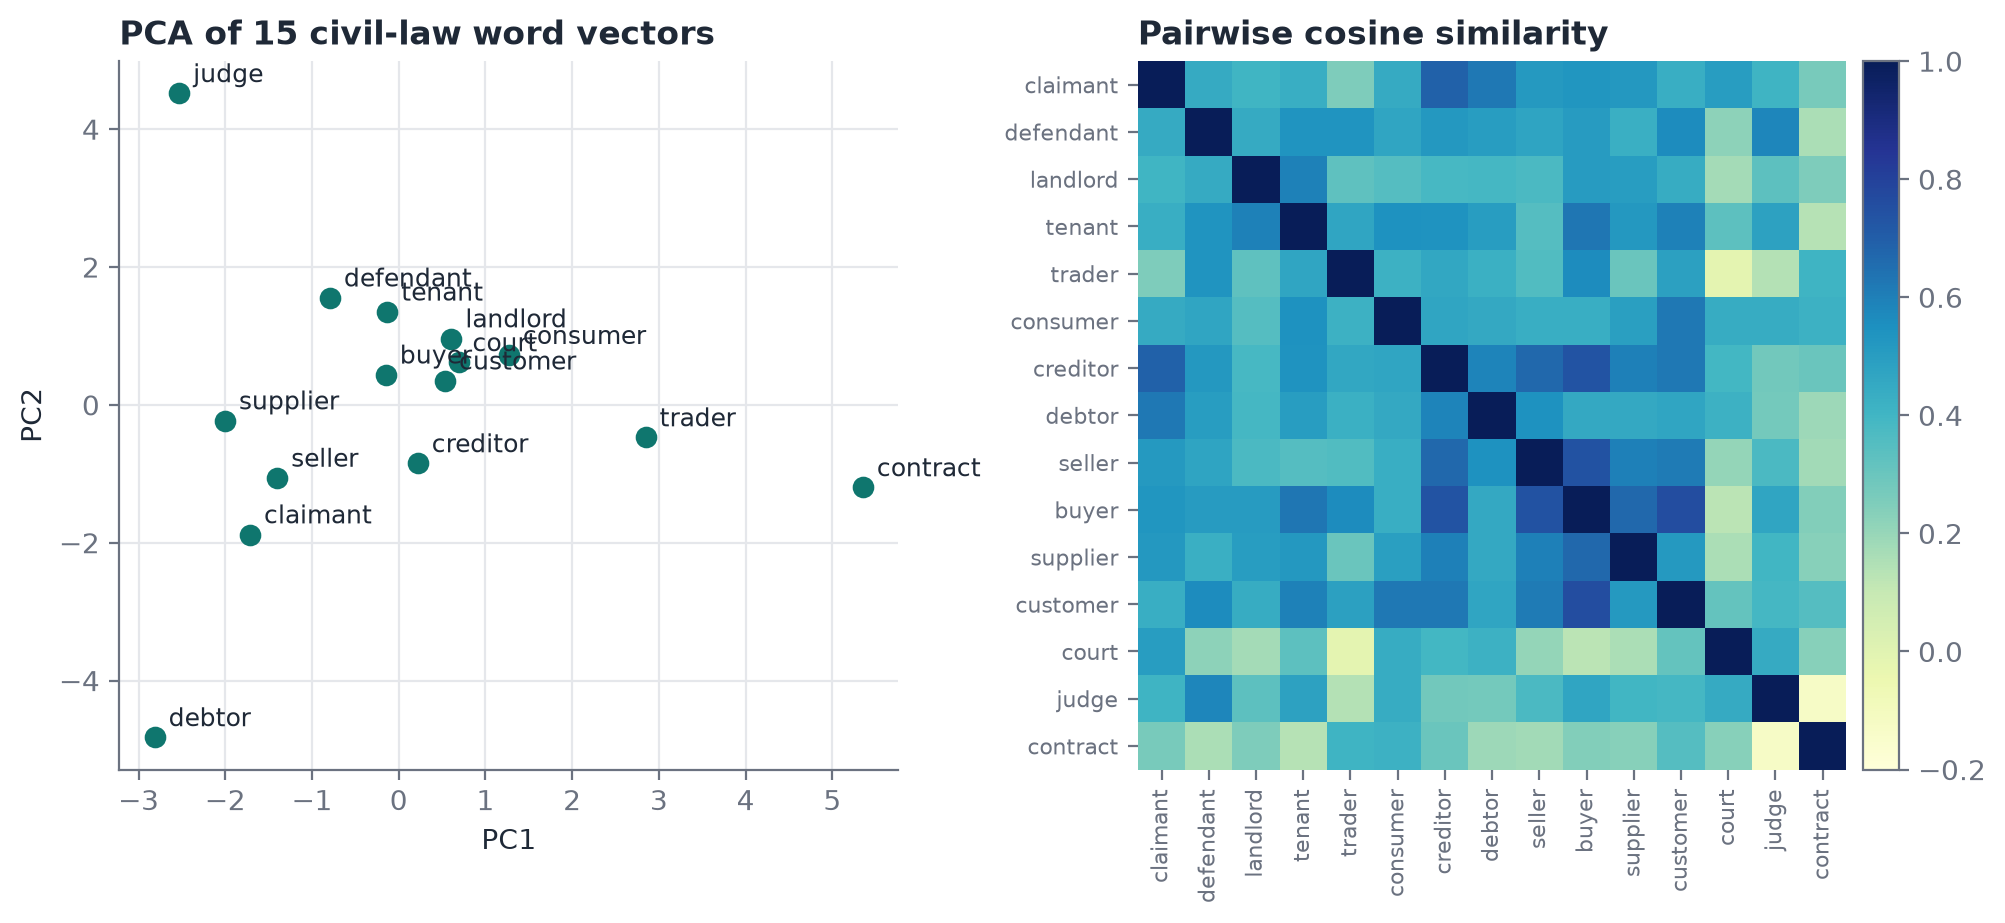
\includegraphics[width=\columnwidth]{fig-skipgram-civil-law.png}
\caption{PCA and cosine matrix of 15 civil-law word vectors, from the saved embeddings.}\label{fig:sg}
\end{figure}

\textbf{Nearest neighbours.} From the \texttt{/train-embed} page with \texttt{claimant defendant landlord tenant} (10,000 epochs, seed 42; loss at epoch 0 4.102625), Table~\ref{tab:nn} and Fig.~\ref{fig:nn}. Pairwise: landlord--tenant 0.59, defendant--tenant 0.54, claimant--defendant 0.44, defendant--landlord 0.44, claimant--tenant 0.43, claimant--landlord 0.40.

\begin{table}[t]
\caption{Five nearest neighbours (cosine).}\label{tab:nn}
\centering\footnotesize\setlength{\tabcolsep}{3pt}
\begin{tabular}{@{}lL{6.6cm}@{}}
\toprule
Word & Neighbours\\
\midrule
claimant & creditor 0.69, remoteness 0.67, limitation 0.67, evidence 0.66, test 0.64\\
defendant & noise 0.69, loser 0.66, authorities 0.64, hearing 0.62, talking 0.62\\
landlord & tenant 0.59, protect 0.59, higher 0.57, thought 0.57, loss 0.56\\
tenant & income 0.67, area 0.66, disputed 0.64, buyer 0.63, price 0.62\\
\bottomrule
\end{tabular}
\end{table}

\begin{figure}[!t]
\centering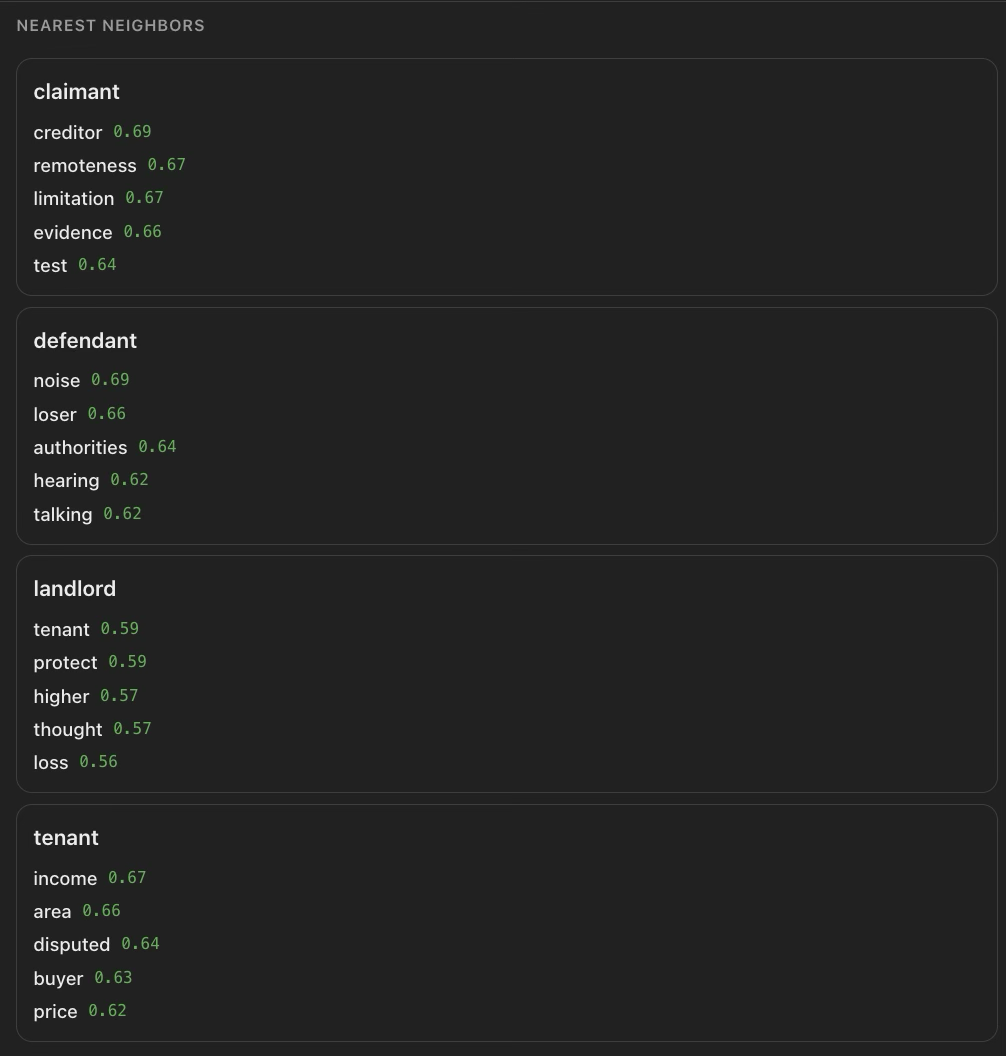
\includegraphics[width=0.5\columnwidth]{pretrain-embed-neighbors.png}
\caption{Nearest neighbours, from the \texttt{/train-embed} page.}\label{fig:nn}
\end{figure}

\textbf{Four seeds: the geometry agrees, the coordinates do not.} Measured on the earlier toy corpus, not yet re-run on the civil-law corpus (Table~\ref{tab:seedtoy}, Fig.~\ref{fig:seedagree}). The learned \emph{function} is stable across seeds; the \emph{weights} are not. So the internal solution is neither unique nor designed, and you cannot read a reason off it. Stability also does not mean correctness: the same analogy error appears on every seed.

\begin{table}[t]
\caption{Seed agreement, Skip-gram, toy corpus (6 seed pairs).}\label{tab:seedtoy}
\centering\footnotesize\setlength{\tabcolsep}{4pt}
\begin{tabular}{@{}lr@{}}
\toprule
Measure & Range\\
\midrule
Cosine of the \emph{same word} across seeds & $-0.28$ to 0.09\\
Correlation of the \emph{pairwise geometry} across seeds & 0.977 to 0.984\\
Analogies correct (our answer key) & 5/7 to 6/7\\
\bottomrule
\end{tabular}
\end{table}

\begin{figure}[!t]
\centering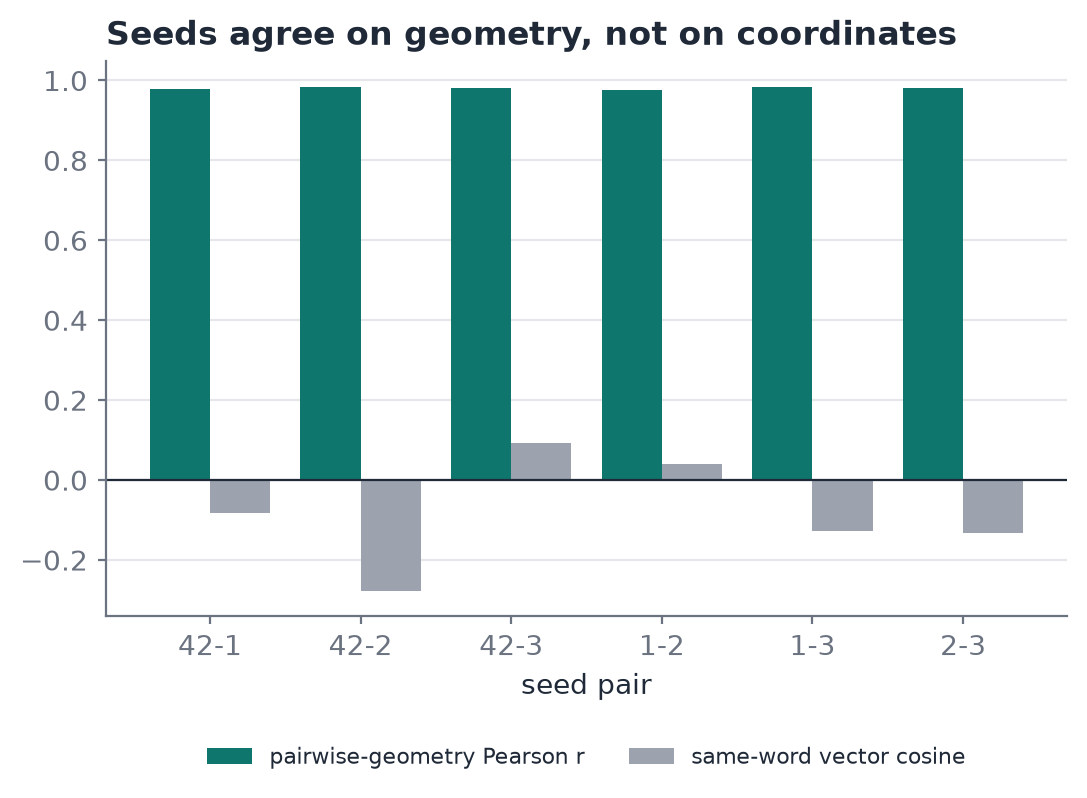
\includegraphics[width=0.72\columnwidth]{fig-seed-agreement.png}
\caption{Seed agreement: geometry agrees, coordinates do not.}\label{fig:seedagree}
\end{figure}

\textbf{Transformer baseline.} 2000 epochs, 2 layers, temperature 1, top-$p$ 0.6, 20 tokens, seed 42, sent as \texttt{2000 1 0.6 2 20} (about 86 minutes); Table~\ref{tab:tf}, Fig.~\ref{fig:sbs}, left. Sample at epoch 2000, prompt ``the claimant is'': \emph{``the claimant is the person who brings a claim. the defendant is the person who answers a claim. the claimant asks''}. \textbf{This loss shows memorisation, not generalisation.} The whole sample is an unbroken stretch of the training text, and as the loss falls the samples turn into copies (Table~\ref{tab:copy}); a token counts as copied if it sits inside a run of 8 or more tokens found verbatim in the training token stream. A superseded 300-epoch baseline, recorded on 2026-10-31 with the three defects present, stalled at a loss of 5.678 (perplexity $\approx$ 292) with domain words in no order; it is kept only as a record.

\begin{table}[t]
\caption{Transformer baseline, 2000 epochs, seed 42.}\label{tab:tf}
\centering\footnotesize\setlength{\tabcolsep}{3pt}
\begin{tabular}{@{}lL{4.6cm}@{}}
\toprule
Measure & Value\\
\midrule
Training text & 256 items (222 definitions + 34 stories)\\
Vocabulary & 937 tokens (1781 BPE merges)\\
Parameters & 87,401\\
Training windows & 5,374 windows of 16 tokens\\
Loss at epoch 0 & 6.868 ($\ln 937=6.843$, a uniform guess)\\
Loss at 100, 300, 500, 1000, 1500 & 4.850, 2.217, 1.051, 0.391, 0.287\\
Lowest logged loss & 0.248 at epoch 1980\\
Final loss, epoch 2000 & 0.2489 (perplexity $\approx$ 1.28)\\
Held-out loss & Not measured: trained on all 256 items\\
\bottomrule
\end{tabular}
\end{table}

\begin{table}[t]
\caption{Generated tokens copied from the training text.}\label{tab:copy}
\centering\footnotesize\setlength{\tabcolsep}{4pt}
\begin{tabular}{@{}lrrr@{}}
\toprule
Epochs & Samples & Copied, mean & Entirely copied\\
\midrule
0--300 & 31 & 0.0\% & 0\\
310--500 & 20 & 5.5\% & 0\\
510--1000 & 50 & 79.7\% & 0\\
1010--1500 & 50 & 99.5\% & 15\\
1510--2000 & 50 & 100\% & 38\\
\bottomrule
\end{tabular}
\end{table}

\textbf{What is measured so far: low loss is not correctness} (Table~\ref{tab:measured}). Fluent samples from earlier in the run state definitions the corpus does not contain, and contradict its definition of a claimant as ``the person who brings a claim'': \emph{``the claimant is the person who owns the home. the tenant is the person who rents the home. the landlord gets''} (epochs 1000 and 1370); \emph{``the claimant is the person who rents the home. the landlord gets the rent. the tenant pays the rent. the''} (epoch 1380). These samples show that this happens, not how often. On held-out stories, a larger configuration ($d{=}64$, 4 heads) does not beat a bigram model on any of the four folds. The Skip-gram result is the same gap in another form: moderate similarity, wrong relation.

\begin{table}[t]
\caption{Measured baselines (no KB, mask or semantic loss).}\label{tab:measured}
\centering\footnotesize\setlength{\tabcolsep}{3pt}
\begin{tabular}{@{}L{2.2cm}L{3.3cm}L{2.5cm}@{}}
\toprule
Baseline & Measure & Value\\
\midrule
Skip-gram, one seed & Role analogies correct & 0 of 5\\
 & landlord--tenant cosine & 0.59\\
Transformer, 2000 epochs, all text & Final loss & 0.2489\\
 & Tokens copied, epochs 1510--2000 & 100\%\\
Transformer, 4-fold held-out stories, 16 runs/config & Test loss, lr 3e-4 / 1e-4 (nats/token) & 5.389$\pm$0.165 / 5.386$\pm$0.174\\
 & Bigram / unigram baseline & 5.290 / 6.012\\
 & Runs beating the bigram, per character & 0 of 16 / 1 of 16\\
\bottomrule
\end{tabular}
\end{table}

\textbf{The reasoning gap.} The objective has no notion of truth: it rewards sounding like the corpus. Weights come from a random start, and XOR and Skip-gram show equal behaviour from unrelated weights. ``Pure emergent, not designed'' means opaque: attention maps show where the model looked, not a justification it could be held to. More layers do not change the objective; whether reasoning emerges at scale is open, and we claim only that nothing in \emph{this} small model asks for it or exposes it. The semantic loss has limits of its own, from the literature: Xu et al.~\cite{xu2018} report that 69.89\% of test predictions satisfied the constraint on grid paths and 55.28\% on preference rankings, large gains but far from complete; a missing rule constrains nothing and a wrong one is trained in; and even with correct constraints, the generalisation benefit comes with a bias toward a suboptimal model~\cite{wang2023}. The two sources of randomness also stay (Table~\ref{tab:rand}). Fixing the seed makes a run repeatable, not justified; greedy decoding removes the draw, but the output is then one fixed point of one seed's distribution. Removing all uncertainty would be the wrong goal anyway, because language has many acceptable continuations and ambiguity is a normal feature of it~\cite{piantadosi,holtzman}.

\begin{table*}[t]
\caption{The two sources of randomness, and what the mechanisms (M1--M5) do to them.}\label{tab:rand}
\centering\footnotesize\setlength{\tabcolsep}{4pt}
\begin{tabular}{@{}L{2.2cm}L{3.4cm}L{6.6cm}L{4.6cm}@{}}
\toprule
Source & Where & What the approach does to it & What is left\\
\midrule
Weight initialisation & Xavier init from the seeded \texttt{rand} (\texttt{matrix.ts}) & The semantic loss constrains outputs, not coordinates, so it adds a term to training that still starts from random weights. The mask, trace and verifier never touch the weights. & Seeds still end at unrelated weights, and may disagree more among allowed tokens~\cite{zombori}\\
Top-$p$ sampling & The draw in \texttt{generateText}, from the same \texttt{rand} & The semantic loss changes the probabilities drawn from, and the mask removes banned tokens before temperature and top-$p$. The draw itself stays. The verifier only checks text after it is drawn. & The next token is still picked at random from what remains in the nucleus\\
\bottomrule
\end{tabular}
\end{table*}

\subsection{One full-length run: $\lambda_s{=}50$ against the CE-only baseline}
\textbf{One seed, one $\lambda_s$, trained on all text. This describes two models; it does not measure an effect of the loss.} $\lambda_s{=}50$ was chosen after 300-epoch trial runs at $\lambda_s\in\{0,2,10,50\}$, simply as the highest value tried. Sent as \texttt{2000 0.8 0.9 2 40 50 42} (about 90 minutes). The control is the same trainer at $\lambda_s{=}0$; its epoch-2000 weights are identical to the baseline's, as are all 210 logged baseline losses. Table~\ref{tab:l50} is read from the saved weights at the 86 training positions where the KB fires (Fig.~\ref{fig:loss}).

\begin{table}[t]
\caption{$\lambda_s{=}50$ vs CE only at the 86 constrained positions.}\label{tab:l50}
\centering\footnotesize\setlength{\tabcolsep}{2.5pt}
\begin{tabular}{@{}llrrrr@{}}
\toprule
Ep. & Model & Sem.\ loss & Banned & $p$(next word) & $p$(own verb)\\
\midrule
300 & CE only & 7.73e-5 & 0.0725 & \textbf{0.045} & \textbf{0.033}\\
 & CE + SL & \textbf{9.85e-6} & \textbf{0.0098} & 0.036 & 0.012\\
600 & CE only & 3.72e-4 & 0.2831 & \textbf{0.339} & \textbf{0.249}\\
 & CE + SL & \textbf{1.34e-5} & \textbf{0.0133} & 0.236 & 0.140\\
1000 & CE only & 2.06e-4 & 0.1647 & 0.739 & 0.612\\
 & CE + SL & \textbf{2.34e-6} & \textbf{0.0023} & \textbf{0.866} & \textbf{0.732}\\
2000 & CE only & 4.58e-5 & 0.0419 & 0.946 & 0.809\\
 & CE + SL & \textbf{6.26e-7} & \textbf{0.0006} & \textbf{0.978} & \textbf{0.841}\\
\bottomrule
\end{tabular}
\end{table}

\begin{figure*}[!t]
\centering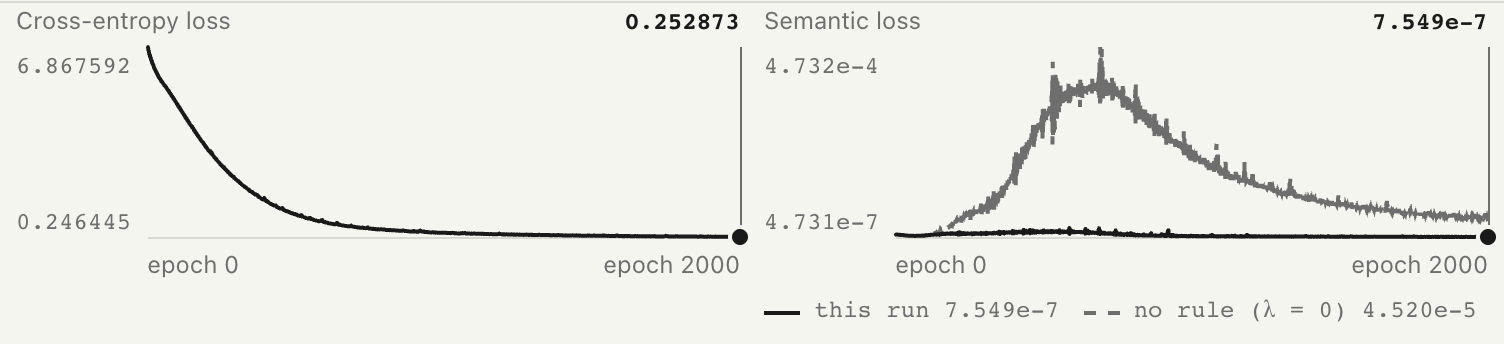
\includegraphics[width=0.72\textwidth]{ns-l50-vs-l0-e2000-loss.png}
\caption{Cross-entropy (left) and semantic loss (right) by epoch, $\lambda_s{=}50$; the $\lambda_s{=}0$ control is dashed and ends at 4.520e-5, against 7.549e-7.}\label{fig:loss}
\end{figure*}

\begin{itemize}
\item \textbf{The banned mass is lower at every epoch above.} At epoch 2000, semantic loss is 73 times lower. The semantic loss logged during training peaks at 4.73e-4 (epoch 689) without the term and at 2.26e-5 (epoch 585) with it.
\item \textbf{The early cost does not last in this run.} Up to about epoch 600 the term also slows the allowed words, including the role's own verb. By epoch 1000 it is ahead on both.
\item \textbf{The training loss costs a little.} Final cross-entropy is 0.2524 against 0.2489; both models copy the training text, so this is not a held-out measure.
\end{itemize}

A rule counts as violated when its banned word's mean $p$ at its trigger pattern is at least 0.02; there are 48 rules (Table~\ref{tab:viol}). Across all 2001 logged epochs, CE only violates at least one rule at 1846 of them, with a maximum of 29 at epoch 529. The neural-symbolic model violates at least one at 175, with a maximum of 3 at epoch 585, and none after epoch 1746. CE only's 7 violations at epoch 2000 are all on the claimant and defendant frames, led by \emph{claimant $\to$ answers} at $p{=}0.124$.

\begin{table}[t]
\caption{Rules violated (of 48) and lifted confirmed / conflict / novel.}\label{tab:viol}
\centering\footnotesize\setlength{\tabcolsep}{3pt}
\begin{tabular}{@{}lrrrr@{}}
\toprule
Epoch & Viol., CE & Viol., CE+SL & Lifted, CE & Lifted, CE+SL\\
\midrule
100 & 0 & 0 & 0 / 0 / 1 & 0 / 0 / 3\\
200 & 5 & 0 & 1 / 6 / 57 & 1 / 1 / 56\\
300 & 5 & 0 & 2 / 8 / 91 & 1 / 2 / 90\\
400 & 23 & 0 & 7 / 32 / 134 & 3 / 9 / 115\\
600 & 26 & 1 & 7 / 43 / 54 & 7 / 18 / 79\\
1000 & 22 & 0 & 8 / 42 / 15 & 7 / 14 / 26\\
1500 & 11 & 0 & 8 / 35 / 5 & 8 / 14 / 8\\
2000 & 7 & 0 & 8 / 32 / 5 & 8 / 15 / 4\\
\bottomrule
\end{tabular}
\end{table}

\textbf{It acts where it fires, and not reliably beyond.} Each role appears in only one of the three definition frames in the corpus, such as \emph{trader} only in ``is a business that''. The compare view probes all 24 role-and-frame contexts with the prompt alone, mask off (Table~\ref{tab:ctx}). Lifting shows the same split: at epoch 2000, conflicts on trained frames fall from 4 to 0; on untrained frames from 28 to 15, but nearly all confident ones ($p\ge0.3$) remain, 9 against 10. These are mostly ``sells'' after ``is a business that'', at $p$ 0.81--0.96 for 6 roles, which suggests the frame, not the role, drives the prediction; that reading is not tested separately. With the prompt ``the claimant is the person who'' (sampling seed 42, $T{=}0.8$, top-$p$ 0.9), both models write the same text with the mask off and on; the verifier finds 2 supported claims and 0 contradicted, and the mask trace shows banned mass at step 0 of 0.3252 for the baseline and 0.0026 for the neural-symbolic model. Screenshots of the run are in Fig.~\ref{fig:nsrun}.

\begin{table}[t]
\caption{Prompt-only probes of all 24 role-and-frame contexts, mask off.}\label{tab:ctx}
\centering\footnotesize\setlength{\tabcolsep}{3pt}
\begin{tabular}{@{}L{2.6cm}rrr@{}}
\toprule
Contexts & Baseline & Neural-symb. & Lower/higher\\
\midrule
8 trained (role's corpus frame) & 0.0959 & 0.0013 & 7 / 1\\
16 untrained (other two frames) & 0.6154 & 0.4975 & 9 / 7\\
of which ``is a business that'', 7 roles & 0.7787 & 0.8331 & 1 / 6\\
\bottomrule
\end{tabular}
\end{table}

\begin{figure}[!t]
\centering
\begin{minipage}[b]{0.45\columnwidth}\centering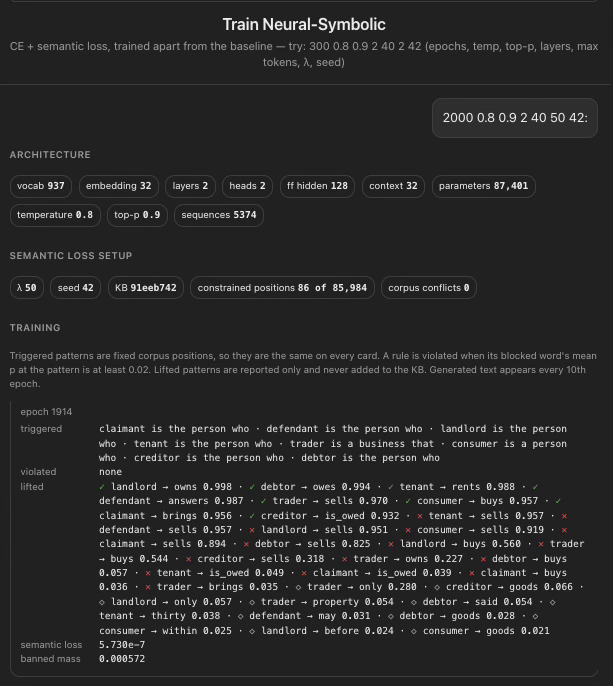
\includegraphics[width=\linewidth]{ns-l50-e2000-epoch-card.png}\\{\scriptsize (a) Epoch 1914}\end{minipage}\hfill
\begin{minipage}[b]{0.53\columnwidth}\centering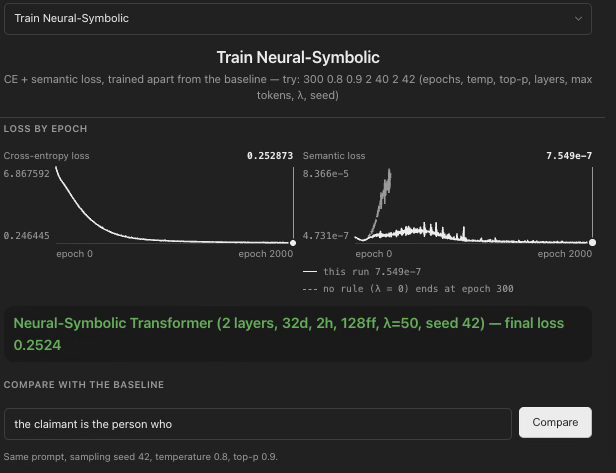
\includegraphics[width=\linewidth]{ns-l50-e2000-loss-compare.png}\\{\scriptsize (b) Loss to epoch 2000}\end{minipage}
\caption{The $\lambda_s{=}50$ run: (a) no rule violated, lifted patterns marked; (b) final loss 0.2524, $\lambda_s{=}0$ control (dashed) to epoch 300 only.}\label{fig:nsrun}
\end{figure}

\subsection{Pre-symbolic transformer vs neural-symbolic run}
Both runs have the same architecture, corpus and seed, and 2000 epochs (Fig.~\ref{fig:sbs}). The left run is the CE-only baseline, sent as \texttt{2000 1 0.6 2 20}, so its samples use temperature 1, top-$p$ 0.6 and 20 tokens. The right run adds the KB and the semantic loss at $\lambda_s{=}50$, and samples at temperature 0.8, top-$p$ 0.9 and 40 tokens. Final cross-entropy is 0.2489 on the left and 0.2524 on the right; on the right, no rule is violated at epoch 2000 (0 of 48).

\begin{figure*}[!tp]
\centering
\begin{minipage}[t]{0.40\textwidth}\centering
{\footnotesize\textbf{Pre-symbolic transformer (CE only)}}\\[3pt]
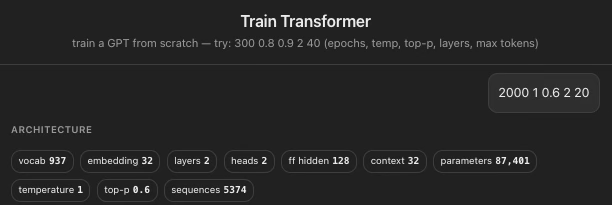
\includegraphics[width=\linewidth]{pretrain-transformer-config.png}\\[2pt]
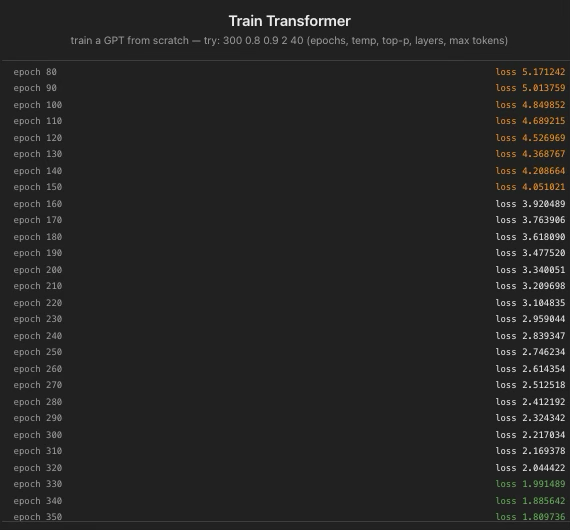
\includegraphics[width=0.78\linewidth]{pretrain-transformer-loss.png}\\[2pt]
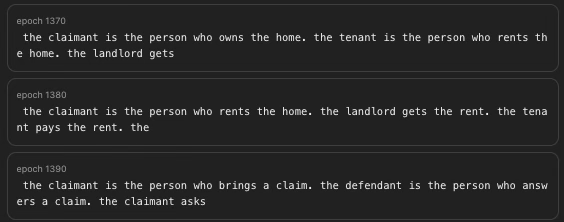
\includegraphics[width=\linewidth]{pretrain-transformer-samples.png}\\[2pt]
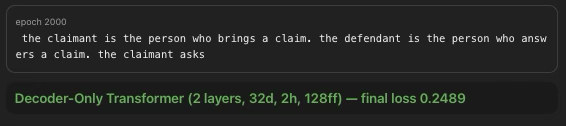
\includegraphics[width=\linewidth]{pretrain-transformer-final.png}
\end{minipage}\hfill
\begin{minipage}[t]{0.57\textwidth}\centering
{\footnotesize\textbf{Neural-symbolic run ($\lambda_s{=}50$)}}\\[3pt]
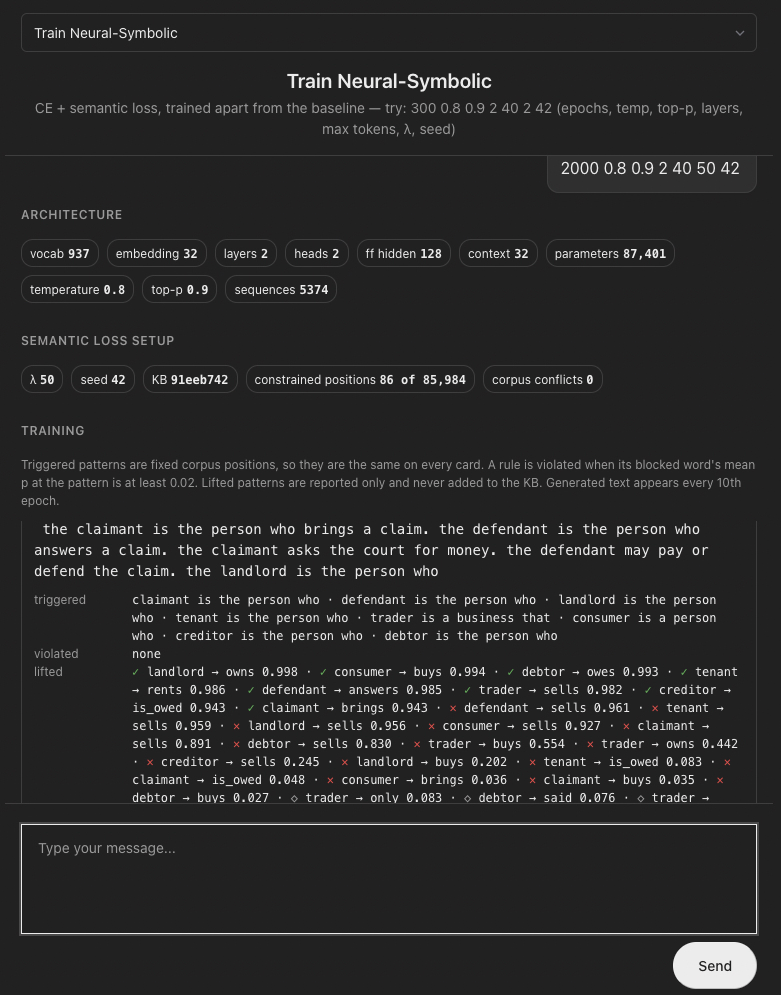
\includegraphics[width=0.49\linewidth]{ns-l50-e2000-demo-epoch.png}\hfill
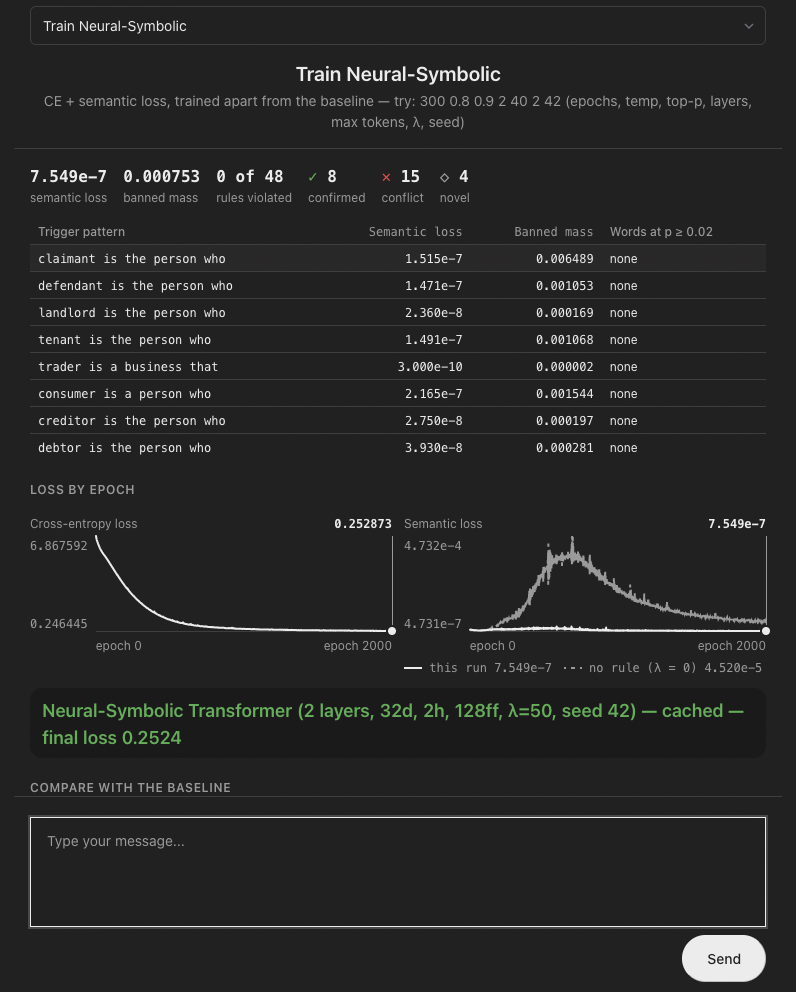
\includegraphics[width=0.49\linewidth]{ns-l50-e2000-demo-dashboard.png}
\end{minipage}
\caption{\textbf{Pre-symbolic transformer vs neural-symbolic run.} Left, top to bottom: architecture, loss to epoch 350, samples at epochs 1370--1390, final loss 0.2489. Right: the live demo after 2000 epochs at $\lambda_s{=}50$, 0 of 48 rules violated.}\label{fig:sbs}
\end{figure*}

\subsection{E2 and E3 at one training seed}
\textbf{One training seed (42), so E2 is partial here; Sec.~\ref{sec:e14} completes it at four seeds.} Everything below was fixed before running. \emph{Models:} the CE-only baseline and the $\lambda_s{=}50$ model, both 2000 epochs. \emph{Prompts:} every role in every definition frame, $8\times3=24$; 8 occur in the training text, and 16 put a role in a frame it never appears in. \emph{Sampling:} seeds 0--49 per prompt, 20 tokens, at $T{=}0.8$, top-$p$ 0.9 and at $T{=}1$, top-$p$ 1. \emph{Mask off:} the processor runs with $\lambda{=}0$ in bias mode, which edits nothing but records \textit{massBefore}; all 4,800 mask-off texts matched plain generation (P2). \emph{Violations:} claims the verifier parsed and found contradicted by the KB; the 95\% Wilson interval treats claims as independent, so it is too narrow, and covers sampling only (Table~\ref{tab:e2}).

\begin{table*}[t]
\caption{E2 at seed 42: contradicted / parsed claims, with the 95\% interval. 400 samples per cell for the training-text prompts and 800 for the others.}\label{tab:e2}
\centering\footnotesize\setlength{\tabcolsep}{5pt}
\begin{tabular}{@{}llllr@{}}
\toprule
Prompts & Model & Mask off, $T$ 0.8, top-$p$ 0.9 & Mask off, $T$ 1, top-$p$ 1 & Mask on, both settings\\
\midrule
8 in the training text & CE only & 7 / 598 (1.2\%, 0.6--2.4\%) & 28 / 578 (4.8\%, 3.4--6.9\%) & 0 / 600, 0 / 578\\
8 in the training text & CE + SL ($\lambda_s{=}50$) & 0 / 600 (0--0.6\%) & 0 / 573 (0--0.7\%) & 0 / 600, 0 / 573\\
16 not in the training text & CE only & 515 / 1,253 (41.1\%, 38.4--43.9\%) & 522 / 1,203 (43.4\%, 40.6--46.2\%) & 0 / 938, 0 / 892\\
16 not in the training text & CE + SL ($\lambda_s{=}50$) & 430 / 1,213 (35.4\%, 32.8--38.2\%) & 420 / 1,159 (36.2\%, 33.5--39.1\%) & 0 / 865, 0 / 839\\
\bottomrule
\end{tabular}
\end{table*}

\begin{table*}[t]
\caption{E3: the two steps where a rule fired.}\label{tab:e3}
\centering\footnotesize\setlength{\tabcolsep}{4pt}
\begin{tabular}{@{}cL{2.6cm}L{4.4cm}L{2.9cm}L{1.2cm}L{1.3cm}L{1.0cm}l@{}}
\toprule
Step & Context ends & Rules fired & Masked tokens & \textit{massBefore}, CE & \textit{massBefore}, $\lambda_s{=}50$ & \textit{massAfter} & Chosen\\
\midrule
0 & the claimant is the person who & 6 bans (answers by R-COUNTER; owns, rents, sells, buys, owes by R-OTHER-DOMAIN), 1 support (brings) & answers, owns, rents, sells, buys, owes & 0.3252 & 0.0026 & 0 & brings\\
10 & the defendant is the person who & 6 bans (brings by R-COUNTER; owns, rents, sells, buys, owes by R-OTHER-DOMAIN), 1 support (answers) & brings, owns, rents, sells, buys, owes & 0.0192 & 0.0002 & 0 & answers\\
\bottomrule
\end{tabular}
\end{table*}

\begin{table*}[t]
\caption{The four arms at seeds 42, 1, 2, 3.}\label{tab:arms}
\centering\footnotesize\setlength{\tabcolsep}{5pt}
\begin{tabular}{@{}L{3.0cm}L{3.2cm}L{3.4cm}L{3.4cm}L{3.0cm}@{}}
\toprule
Arm ($\lambda_s$, mask) & Banned mass, 86 positions, mask off & Contradicted, 16 untrained prompts, $T$ 0.8 & Contradicted claims the mask did not cover & Held-out CE\\
\midrule
CE only & 0.024--0.049 & 35.4--47.9\% & --- & not measured (no held-out split)\\
CE + semantic loss & 0.008--0.016 & 31.3--45.7\% & --- & not measured\\
CE + mask & --- (mask edits after the network) & 0\% at 3 seeds, 17.8\% at seed 1 & 167 at seed 1, all ``owed'' & not measured\\
CE + semantic loss + mask & --- & 0\% at 3 seeds, 11.6\% at seed 1 & 111 at seed 1, all ``owed'' & not measured\\
\bottomrule
\end{tabular}
\end{table*}

\begin{table*}[t]
\caption{E4 per seed (42, 1, 2, 3).}\label{tab:e4}
\centering\footnotesize\setlength{\tabcolsep}{5pt}
\begin{tabular}{@{}lll@{}}
\toprule
Measure & $\lambda_s{=}0$ & $\lambda_s{=}2$\\
\midrule
Banned mass, 86 constrained positions, mask off & 0.042, 0.049, 0.024, 0.029 & 0.010, 0.016, 0.009, 0.008\\
Banned mass, 8 training-text prompts & 0.096, 0.087, 0.036, 0.076 & 0.021, 0.024, 0.015, 0.014\\
Banned mass, 16 untrained prompts & 0.615, 0.451, 0.734, 0.663 & 0.529, 0.432, 0.708, 0.532\\
Frequency-matched control set, untrained prompts & 0.0009, 0.0052, 0.0003, 0.0039 & 0.0079, 0.0058, 0.0000, 0.0013\\
Contradicted claims, untrained prompts, mask off, $T$ 0.8 & 41.1\%, 35.4\%, 47.9\%, 46.0\% & 32.6\%, 31.3\%, 45.7\%, 40.1\%\\
$H(q_A)$ at constrained positions (bits) & 0.127, 0.209, 0.167, 0.185 & 0.125, 0.199, 0.152, 0.159\\
Perplexity where no rule fires (training text) & 1.283, 1.281, 1.268, 1.266 & 1.281, 1.281, 1.264, 1.266\\
Final training cross-entropy & 0.2489, 0.2471, 0.2374, 0.2358 & 0.2478, 0.2471, 0.2340, 0.2356\\
\bottomrule
\end{tabular}
\end{table*}

\begin{itemize}
\item \textbf{With the mask on, no parsed claim contradicts the KB:} 0 of 5,885 claims across all eight cells. At this seed that checks the implementation (P1), not the model.
\item \textbf{With the mask off, the CE-only model contradicts the KB:} 1.2\% at $T{=}0.8$ and 4.8\% at $T{=}1$ on the 8 training-text prompts, 41--43\% on the 16 others.
\item \textbf{On the training-text prompts, the $\lambda_s{=}50$ model made no contradicted claims in 1,173.} Its mean \textit{massBefore} where a rule fired was 0.0010 and 0.0028, against 0.0739 and 0.0771 for CE only. These are training contexts, at one seed.
\item \textbf{On the other 16 prompts, it still contradicts the KB in 35--36\% of claims.} At $T{=}0.8$, 315 of its 430 contradicted claims are ``sells'' after ``is a business that'', the verb of trader, the one role trained in that frame; another 100 are ``buys'' after ``is a person who'', the verb of consumer. CE only does the same: 296 and 126 of its 515. Each model completes a frame with the verb of the role trained in it, whatever the role.
\item \textbf{On those 16 prompts, the mask mostly turns contradicted claims into unknown ones.} For CE only at $T{=}0.8$, unknown claims rise from 50 to 443 and supported claims fall from 688 to 495.
\end{itemize}

\textbf{E3: one full trace.} Prompt ``the claimant is the person who'', sampling seed 42, $T{=}0.8$, top-$p$ 0.9, mask on. Both models generated ``the claimant is the person who brings a claim. the defendant is the person who answers a claim. the claimant asks the court for''. The verifier parsed 2 claims, both supported. A rule fired at 2 of the 20 steps (Table~\ref{tab:e3}); at the other 18 the mask changed nothing.

\subsection{E1 and E4: four training seeds}\label{sec:e14}
\begin{table}[t]
\caption{E1, $\lambda_s{=}0$, six seed pairs.}\label{tab:e1}
\centering\footnotesize\setlength{\tabcolsep}{3pt}
\begin{tabular}{@{}L{4.6cm}L{3.3cm}@{}}
\toprule
Measure & Range over seed pairs\\
\midrule
Final training CE, per seed & 0.2358, 0.2374, 0.2471, 0.2489\\
Weight cosine (87,401 parameters) & 0.023--0.071\\
Weight L2 distance (norms 82.8--83.8) & 113.5--115.9\\
Same top-1 word, 8 training-text prompts & 8 of 8 for every pair\\
Same top-1 word, 16 held-out prompts & 50--69\% (mean 58\%)\\
JS of next-word dist., training-text prompts & 0.052--0.060 bits\\
JS, held-out prompts & 0.23--0.34 bits\\
Cosine of centred logits, held-out prompts & 0.15--0.20\\
\bottomrule
\end{tabular}
\end{table}

\begin{table}[t]
\caption{E2 at four seeds, CE-only models, mask off: contradicted / parsed claims.}\label{tab:e2seeds}
\centering\footnotesize\setlength{\tabcolsep}{3pt}
\begin{tabular}{@{}llll@{}}
\toprule
Seed & Train prompts, $T$ 0.8 & Untrained, $T$ 0.8 & Untrained, $T$ 1\\
\midrule
42 & 7 / 598 (1.2\%) & 515 / 1,253 (41.1\%) & 522 / 1,203 (43.4\%)\\
1 & 4 / 593 (0.7\%) & 408 / 1,151 (35.4\%) & 427 / 1,114 (38.3\%)\\
2 & 0 / 600 (0\%) & 628 / 1,310 (47.9\%) & 601 / 1,277 (47.1\%)\\
3 & 7 / 593 (1.2\%) & 572 / 1,243 (46.0\%) & 574 / 1,200 (47.8\%)\\
\bottomrule
\end{tabular}
\end{table}

\begin{table}[t]
\caption{E4 across the six seed pairs.}\label{tab:e4pairs}
\centering\footnotesize\setlength{\tabcolsep}{3pt}
\begin{tabular}{@{}L{3.6cm}L{2.2cm}L{2.2cm}@{}}
\toprule
Measure & $\lambda_s{=}0$ & $\lambda_s{=}2$\\
\midrule
JS of $(P_A,1{-}P_A)$, constrained (mean) & 7.5e-3 (5.4e-3 to 1.0e-2) & 2.5e-3 (1.9e-3 to 3.2e-3)\\
JS of $q_A$, constrained (mean) & 0.0153 & 0.0149\\
Weight cosine & 0.023--0.071 & 0.025--0.071\\
JS of next-word dist., held-out (mean) & 0.30 bits & 0.38 bits\\
Same top-1 word, held-out (mean) & 58\% & 61\%\\
\bottomrule
\end{tabular}
\end{table}

\textbf{Eight models: $\lambda_s\in\{0,2\}$ $\times$ training seeds 42, 1, 2 and 3, all 2000 epochs, trained on all text}, 68 to 81 minutes each. The measures were fixed before the last run finished. At seed 42 the $\lambda_s{=}0$ model has exactly the baseline's weights (L2 distance 0). \emph{Held-out prompts:} the 16 role-and-frame prompts that never occur in the training text, the only held-out data. \emph{Constrained positions:} the 86 training positions where a rule fires. \emph{Four seeds:} with 4 of 4 seeds in the same direction, a paired sign-flip test cannot go below $p{=}0.125$, so ``lower at every seed'' is not a significance claim. Table~\ref{tab:arms} summarises the four arms.

\textbf{E1 (P4): similar loss, unrelated weights, and different behaviour where training gave no data} (Table~\ref{tab:e1}). Two vectors of norm 83 at right angles are about 118 apart, so the weight vectors are close to unrelated. Part of this is symmetry (hidden units can be permuted), which is why the comparison also uses outputs. On text they trained on, all four seeds pick the same next word; on prompts outside it they pick different words a third to a half of the time. \textbf{P4 is supported.}

\textbf{E2 at four seeds (P1, P3)} (Table~\ref{tab:e2seeds}). \textbf{P3 is supported:} every seed contradicts the KB on 35--48\% of claims from untrained prompts. \textbf{P1 is not supported as implemented.} With the mask on, 514 of 23,664 parsed claims across all 16 mask-on cells contradict the KB. Ten cells have none, and 509 of the 514 come from seed 1 (both values of $\lambda_s$). Every one is the same case: the model writes ``\dots\ is a business that \textbf{owed} money''. The verifier reads a bare ``owed'' after a frame as \emph{is owed}, but the mask bans ``owed'' only after ``\dots\ that \textbf{is}'', so the bare form is never masked. The mask and the verifier disagree on one surface form; the grammatical reading of ``that owed money'' is closer to \emph{owes}, which the KB also bans for these roles. The fix belongs in the mask or the verifier and would change the E2 numbers, so it is left for review.

\textbf{E4 (P5, P6, P7):} $\lambda_s{=}2$ against $\lambda_s{=}0$ at the same seed (Tables~\ref{tab:e4} and~\ref{tab:e4pairs}).

\begin{itemize}
\item \textbf{P5 is supported on training positions:} banned mass at the 86 constrained positions is 2.6 to 4.3 times lower at every seed, and lower on the 8 training-text prompts at every seed. On the 16 untrained prompts it is also lower at every seed, but by 0.02--0.13 out of 0.45--0.73, and contradicted claims fall by 2 to 9 points. The frequency-matched control set gets almost no mass in either arm, so the banned mass is specific to the banned verbs.
\item \textbf{P6 is supported on constrained positions:} seeds disagree about three times less on how much mass goes to allowed words, while their disagreement among allowed words ($q_A$) is unchanged, as predicted. $H(q_A)$ falls by 2--14\%, which is not collapse onto one word. Weight cosine stays near zero. On held-out prompts the seeds disagree slightly \emph{more} with the loss (0.38 against 0.30 bits), so the reduction stays where the rules fire.
\item \textbf{P7 is not testable here as stated.} On training text where no rule fires, perplexity does not rise (equal or lower at every seed). That is fit, not held-out perplexity, which needs the held-out split.
\item \textbf{Overall:} at $\lambda_s{=}2$, the loss removes banned mass where rules fire, at no measured cost, and barely changes behaviour on contexts it never trained on. This repeats the full-length $\lambda_s{=}50$ run, now across four seeds.
\end{itemize}

%======================================================================
\section{Conclusion}
Three findings hold across seeds. \textbf{Where the constraint is trained, it holds}, at a small cost in training loss. \textbf{Beyond it, the rule does not transfer}: on unseen frames the model follows the frame, not the KB. \textbf{A guarantee covers only what its rules cover}, as the ``owed'' gap shows. Limits: one small model, a hand-written KB, four seeds, and no held-out text split, held-out KB or held-out cross-entropy yet.

\textbf{Related work and positioning.} \emph{Constraints in the loss or output layer:} the semantic loss~\cite{xu2018} is the term M5 adapts; semantic probabilistic layers~\cite{ahmed2022} build consistency into the output layer and train through it, whereas this design keeps loss and mask separate; the pseudo-semantic loss~\cite{ahmed2023} extends the idea to autoregressive models and is the precedent above. \emph{Constrained decoding:} NeuroLogic decoding~\cite{lu2021} searches with lexical constraints, and grammar-constrained decoding~\cite{geng2023} restricts output to a grammar; both act only at decoding, and the M1 mask is simpler than either, a per-token ban with no lookahead. \emph{LLMs with theorem provers:} Explanation-Refiner~\cite{quan2024} uses a theorem prover to verify natural-language explanations and feed corrections back to an LLM; the M4 verifier is a far weaker check, a pattern parser and forward chaining over a small hand-written KB.

\textbf{The same principle on any LLM.} Sheth et al.~\cite{sheth2023} call systems in which an LLM hands sub-tasks to symbolic solvers \emph{federated pipelines}. Here the KB is the solver, and the three access points of Fig.~\ref{fig:pipe} become three levels of API access. With open weights, the semantic loss applies in fine-tuning. Where an API exposes logits or a logit bias, the allowed set can mask decoding. With text only, the verifier returns contradicted claims for regeneration, the verify-and-refine loop of Explanation-Refiner~\cite{quan2024,quan2025} and LLM-Modulo~\cite{llmmodulo}. This extension is designed, not built.

\textbf{Towards neurosymbolic world models.} \emph{A proposed direction; none of this has been done, and this repository contains no robotics.} \emph{Objective 1 (foundations):} move the same two-stage pipeline from token-level constraints on a toy language model to constraints on a pretrained LLM that writes action models (PDDL preconditions and effects). A planner or validator such as VAL~\cite{val}, plus an entailment-based faithfulness check~\cite{quan2024,quan2025}, would take the verifier's role, with localised repair; GPT-4o's PDDL was 96.1\% parseable but 24.8\% correct~\cite{planetarium}. O1 also tests whether world models follow plausibility over validity, like the frame effect above, and whether steering or circuit methods~\cite{valentino2026,kim2025} reduce it. \emph{Objective 2 (controller):} the advert's controller ``will simulate actions and verify constraints to trigger automated error recovery''. That is the same split: a world model trained to respect constraints corresponds to the semantic-loss stage, and a controller that verifies constraints before acting corresponds to the mask and verifier stage. A slow symbolic layer sets subgoals and constraints; a fast controller rolls out an action-conditioned tactile model~\cite{mandil,nazari2022} and checks constraints on predicted states, so a predicted violation triggers replanning before failure, compared with post-failure recovery~\cite{reflect}. The main risk is the one the demo exposed: a wrong or missing rule enters training and decoding at once. So every rule stays traceable to a proof, and where formalisation fails the verifier says \emph{unknown}.

\begin{thebibliography}{99}
\scriptsize
\setlength{\itemsep}{0pt}
%BIB-START
\bibitem{liberopro} X.~Zhou \emph{et al.}, ``LIBERO-PRO: Towards robust and fair evaluation of vision-language-action models beyond memorization,'' arXiv:2510.03827, 2025.
\bibitem{duggan} T.~Duggan \emph{et al.}, ``The price is not right: Neuro-symbolic methods outperform VLAs on structured long-horizon manipulation tasks,'' in \emph{Proc. ICRA}, 2026.
\bibitem{sheth2023} A.~Sheth, K.~Roy, and M.~Gaur, ``Neurosymbolic artificial intelligence (why, what, and how),'' \emph{IEEE Intell. Syst.}, vol.~38, no.~3, pp.~56--62, 2023.
\bibitem{sheth2022} A.~Sheth, M.~Gaur, K.~Roy, R.~Venkataraman, and V.~Khandelwal, ``Process knowledge-infused AI: Towards user-level explainability, interpretability, and safety,'' arXiv:2206.13349, 2022.
\bibitem{roy2022} K.~Roy, M.~Gaur, Q.~Zhang, and A.~Sheth, ``Process knowledge-infused learning for suicidality assessment on social media,'' arXiv:2204.12560, 2022.
\bibitem{xu2018} J.~Xu, Z.~Zhang, T.~Friedman, Y.~Liang, and G.~Van den Broeck, ``A semantic loss function for deep learning with symbolic knowledge,'' in \emph{Proc. ICML}, 2018.
\bibitem{ahmed2023} K.~Ahmed, K.-W.~Chang, and G.~Van den Broeck, ``A pseudo-semantic loss for autoregressive models with logical constraints,'' in \emph{Proc. NeurIPS}, 2023.
\bibitem{w3cj} w3cj, ``how-llms-work'' (reference architecture), GitHub, \url{https://github.com/w3cj/how-llms-work}.
\bibitem{weizenbaum} J.~Weizenbaum, ``ELIZA,'' \emph{Commun. ACM}, vol.~9, no.~1, 1966.
\bibitem{sennrich} R.~Sennrich, B.~Haddow, and A.~Birch, ``Neural machine translation of rare words with subword units,'' in \emph{Proc. ACL}, 2016.
\bibitem{rumelhart} D.~E.~Rumelhart, G.~E.~Hinton, and R.~J.~Williams, ``Learning representations by back-propagating errors,'' \emph{Nature}, vol.~323, 1986.
\bibitem{mikolova} T.~Mikolov, K.~Chen, G.~Corrado, and J.~Dean, ``Efficient estimation of word representations in vector space,'' arXiv:1301.3781, 2013.
\bibitem{mikolovb} T.~Mikolov, I.~Sutskever, K.~Chen, G.~Corrado, and J.~Dean, ``Distributed representations of words and phrases and their compositionality,'' in \emph{Proc. NeurIPS}, 2013.
\bibitem{vaswani} A.~Vaswani \emph{et al.}, ``Attention is all you need,'' in \emph{Proc. NeurIPS}, 2017.
\bibitem{ba2016} J.~L.~Ba, J.~R.~Kiros, and G.~E.~Hinton, ``Layer normalization,'' arXiv:1607.06450, 2016.
\bibitem{kingma} D.~P.~Kingma and J.~Ba, ``Adam: A method for stochastic optimization,'' in \emph{Proc. ICLR}, 2015.
\bibitem{vankrieken} E.~van Krieken, P.~Minervini, E.~Ponti, and A.~Vergari, ``On the independence assumption in neurosymbolic learning,'' in \emph{Proc. ICML}, 2024.
\bibitem{ahmed2022} K.~Ahmed, S.~Teso, K.-W.~Chang, G.~Van den Broeck, and A.~Vergari, ``Semantic probabilistic layers for neuro-symbolic learning,'' in \emph{Proc. NeurIPS}, 2022.
\bibitem{zombori} Z.~Zombori, A.~Rissaki, K.~Szab\'o, W.~Gatterbauer, and M.~Benedikt, ``Towards unbiased exploration in partial label learning,'' \emph{JMLR}, vol.~25, no.~412, 2024.
\bibitem{wang2023} K.~Wang, H.~He, T.~D.~Nguyen, P.~Kumar, and D.~Roth, ``On regularization and inference with label constraints,'' in \emph{Proc. ICML}, 2023.
\bibitem{piantadosi} S.~T.~Piantadosi, H.~Tily, and E.~Gibson, ``The communicative function of ambiguity in language,'' \emph{Cognition}, vol.~122, no.~3, 2012.
\bibitem{holtzman} A.~Holtzman, J.~Buys, L.~Du, M.~Forbes, and Y.~Choi, ``The curious case of neural text degeneration,'' in \emph{Proc. ICLR}, 2020.
\bibitem{lu2021} X.~Lu, P.~West, R.~Zellers, R.~Le~Bras, C.~Bhagavatula, and Y.~Choi, ``NeuroLogic decoding: (Un)supervised neural text generation with predicate logic constraints,'' in \emph{Proc. NAACL}, 2021.
\bibitem{geng2023} S.~Geng, M.~Josifoski, M.~Peyrard, and R.~West, ``Grammar-constrained decoding for structured NLP tasks without finetuning,'' in \emph{Proc. EMNLP}, 2023.
\bibitem{quan2024} X.~Quan, M.~Valentino, L.~A.~Dennis, and A.~Freitas, ``Verification and refinement of natural language explanations through LLM-symbolic theorem proving,'' in \emph{Proc. EMNLP}, 2024, pp.~2933--2958.
\bibitem{quan2025} X.~Quan, M.~Valentino, L.~A.~Dennis, and A.~Freitas, ``Faithful and robust LLM-driven theorem proving for NLI explanations,'' in \emph{Proc. ACL}, 2025.
\bibitem{llmmodulo} S.~Kambhampati \emph{et al.}, ``LLMs can't plan, but can help planning in LLM-Modulo frameworks,'' in \emph{Proc. ICML}, 2024.
\bibitem{val} R.~Howey, D.~Long, and M.~Fox, ``VAL: Automatic plan validation, continuous effects and mixed initiative planning using PDDL,'' in \emph{Proc. ICTAI}, 2004, pp.~294--301.
\bibitem{planetarium} M.~Zuo \emph{et al.}, ``Planetarium: A rigorous benchmark for translating text to structured planning languages,'' in \emph{Proc. NAACL}, 2025.
\bibitem{valentino2026} M.~Valentino, G.~Kim, D.~Dalal, Z.~Zhao, and A.~Freitas, ``Mitigating content effects on reasoning in language models through fine-grained activation steering,'' in \emph{Proc. AAAI}, 2026.
\bibitem{kim2025} G.~Kim, M.~Valentino, and A.~Freitas, ``Reasoning circuits in language models: A mechanistic interpretation of syllogistic inference,'' in \emph{Findings of ACL}, 2025.
\bibitem{mandil} W.~Mandil, K.~Nazari, and A.~Ghalamzan~E, ``Action conditioned tactile prediction: A case study on slip prediction,'' arXiv:2205.09430, 2022.
\bibitem{nazari2022} K.~Nazari, W.~Mandil, and A.~Ghalamzan~E, ``Proactive slip control by learned slip model and trajectory adaptation,'' arXiv:2209.06019, 2022.
\bibitem{reflect} Z.~Liu, A.~Bahety, and S.~Song, ``REFLECT: Summarizing robot experiences for failure explanation and correction,'' in \emph{Proc. CoRL}, 2023.
%BIB-END
\end{thebibliography}

\end{document}
